%!TEX output_directory = aux

\documentclass[11pt,a4paper]{article}

\usepackage[english]{babel}

\usepackage[most]{tcolorbox}

\usepackage{algorithm}
\usepackage{algpseudocode}

% ---- FONT & MICROTYPOGRAPHY ----
\usepackage[utf8]{inputenc}
\usepackage[T1]{fontenc}
\usepackage{microtype}
\usepackage{moresize}

% ---- FORMATTING ----
\usepackage{csquotes,textcase,xspace}

% ---- PAGE LAYOUT ----
\usepackage{geometry}
\geometry{top=2.5cm,bottom=2cm,inner=2cm,outer=2cm,footnotesep=7mm plus 4pt minus 4pt}
\usepackage{setspace}
\setstretch{1.1}

% ---- GRAPHIQUE ----
\usepackage{graphicx}
\usepackage{adjustbox} 
\usepackage{xcolor}
\usepackage[font=small,labelfont=bf,labelsep=space]{caption}
\usepackage{subfigure}
\captionsetup{width=0.9\textwidth,font={small,stretch=1.1}}
\addto\captionsenglish{\renewcommand{\figurename}{Fig.}}
\addto\captionsenglish{\renewcommand{\tablename}{Tab.}}
\definecolor{JoliBleu}{rgb}{0,0.55,0.55}
\definecolor{JoliVert}{rgb}{0.15,0.6,0}
\definecolor{JoliRouge}{rgb}{0.86,0.08,0}
\definecolor{JoliJaune}{rgb}{1,0.75,0}
\definecolor{JoliGris}{rgb}{0.52,0.52,0.51}
\definecolor{myblue}{RGB}{26, 77, 116}
\definecolor{myorange}{RGB}{181, 116, 30}
\definecolor{mydarkorange}{RGB}{166, 88, 0}
\definecolor{mygreen}{RGB}{21, 124, 80}
\definecolor{myblack}{RGB}{43, 65, 82}
\definecolor{myred}{rgb}{0.5, 0.0, 0.13}

% ---- SECTIONING ----
\usepackage{titlesec}
\titleformat{\section}[block]{\Large\boldmath\bfseries}{\thesection}{1em}{}
\titleformat{\subsection}[block]{\large\boldmath\bfseries}{\thesubsection}{0.5em}{}
\usepackage{appendix}
\renewcommand{\setthesection}{\Alph{section}}
\renewcommand{\restoreapp}{}
\makeatletter
\renewcommand{\theequation}{\thesection.\arabic{equation}}
\@addtoreset{equation}{section}
\makeatother

% ---- FOOTERS HEADERS ----
\usepackage[bottom]{footmisc}
\usepackage{fancyhdr}

% ---- TABLE OF CONTENTS ----
\usepackage{titletoc}
\setcounter{tocdepth}{3}

% ---- BIBLIOGRAPHY ----
\usepackage[nosort]{cite}
\bibliographystyle{JHEP}
\newcommand{\eprint}[1]{{\href{http://arxiv.org/abs/#1}{\texttt{[#1]}}}}
\newcommand{\eprintN}[1]{{\href{http://arxiv.org/abs/#1}{\texttt{#1 [hep-th]}}}}
\newcommand{\doi}[2]{\href{http://dx.doi.org/#2}{#1}}

% ---- HYPER REF ----
\usepackage{hyperref}
\hypersetup{colorlinks=true,
        pdfstartview=FitV,
        linkcolor= mydarkorange,
        citecolor= mydarkorange, 
        urlcolor= JoliGris!60!black,
        hypertexnames=false,
        linktoc=page}

% ---- TIKZ ----
\usepackage{tikz}
\usepackage{tcolorbox}
\usetikzlibrary{calc}
\usetikzlibrary{shapes.geometric, arrows.meta, positioning}

% Définition des couleurs modernes
\definecolor{deepblue}{RGB}{41, 128, 185}
\definecolor{lightblue}{RGB}{174, 214, 241}
\definecolor{emerald}{RGB}{46, 204, 113}
\definecolor{lightemerald}{RGB}{212, 245, 227}
\definecolor{coral}{RGB}{231, 76, 60}
\definecolor{lightcoral}{RGB}{250, 215, 212}
\definecolor{charcoal}{RGB}{52, 73, 94}
\definecolor{lightgray}{RGB}{150, 150, 150}

% Styles épurés et modernes
\tikzstyle{startstop} = [
ellipse, 
minimum width=3cm, 
minimum height=1cm, 
text centered, 
draw=charcoal, 
fill=lightgray,
line width=1.2pt,
font=\sffamily\small\bfseries
]

\tikzstyle{process} = [
rectangle, 
minimum width=5.5cm, 
minimum height=1.1cm, 
text centered,
draw=myblue, 
fill=lightblue,
line width=1pt,
rounded corners=2pt,
font=\sffamily\small
]

\tikzstyle{decision} = [
rectangle, 
minimum width=3.2cm, 
minimum height=1.cm, 
text centered, 
draw=myorange, 
fill=myorange!20,
line width=1pt,
font=\sffamily\small\bfseries,
aspect=1.3
]

\tikzstyle{arrow} = [
thick,
->,
>=Stealth,
color=charcoal,
line width=1.5pt
]

\tikzstyle{arrow_label} = [
font=\sffamily\small\bfseries,
color=charcoal
]

% ---- MATHS ----
\usepackage{amsmath,amssymb,amsfonts,dsfont}
\usepackage{mathrsfs}
\usepackage{physics}
\usepackage{ytableau}
\ytableausetup{boxsize=1.1em,centertableaux}
\usepackage{stmaryrd}
\usepackage{nicefrac}
\allowdisplaybreaks[1]
% \usepackage{bbold}
\usepackage{cases}
\usepackage{bm}
\usepackage{bbm}

% ---- TABLES ----
\usepackage{multirow}
\usepackage{booktabs}
\usepackage{pdflscape}
\usepackage{array}
\usepackage{arydshln}

% ---- ENUMERATION ----
\usepackage[shortlabels]{enumitem}

% ---- MATHS COMMANDS ----
\newcommand{\A}{\ensuremath{\mathcal{A}}\xspace}
\newcommand{\F}{\ensuremath{\mathcal{F}}\xspace}
\renewcommand{\H}{\ensuremath{\mathcal{H}}\xspace}
\newcommand{\M}{\ensuremath{\mathcal{M}}\xspace}
\renewcommand{\P}{\ensuremath{\mathcal{P}}\xspace}
\newcommand{\J}{\ensuremath{\mathcal{J}}\xspace}
\renewcommand{\d}{\ensuremath{\mathrm{d}}\xspace}
\renewcommand{\H}{\ensuremath{\mathcal{H}}\xspace}
\newcommand{\SO}{\ensuremath{\mathrm{SO}}\xspace}
\renewcommand{\O}{\ensuremath{\mathrm{O}}\xspace}
\newcommand{\SL}{\ensuremath{\mathrm{SL}}\xspace}
\newcommand{\Odd}{\ensuremath{\mathrm{O}(d,d)}\xspace}
\newcommand{\odd}{\ensuremath{\mathfrak{o}(d,d)}\xspace}
\renewcommand{\Tr}[1]{\ensuremath{\mathrm{Tr}\left(#1\right)}\xspace}
\newcommand{\vol}{{\,\rm vol}}
\def\sst#1{{\scriptscriptstyle #1}}


\def\bbar#1{\bar{\bar{#1}}}

\newcommand{\cN}{{\cal N}}
\newcommand{\cA}{{\cal A}}
%\newcommand{\Tr}{\mbox{Tr}}
%\newcommand{\tr}{\mbox{tr}}
\newcommand{\cZ}{{\cal Z}}


\newcommand{\bK}{{\bar{K}}}
\newcommand{\bL}{{\bar{L}}}
\newcommand{\bM}{{\bar{M}}}
\newcommand{\bN}{{\bar{N}}}
\newcommand{\bP}{{\bar{P}}}
\newcommand{\bQ}{{\bar{Q}}}
\newcommand{\bR}{{\bar{R}}}
\newcommand{\bS}{{\bar{S}}}
\newcommand{\bk}{{\bar{k}}}
\newcommand{\bl}{{\bar{l}}}
\newcommand{\bzero}{{\bar{0}}}
\newcommand{\balpha}{{\bar{\alpha}}}
\newcommand{\bbeta}{{\bar{\beta}}}

\def\dA{{\dot{A}}}
\def\dB{{\dot{B}}}
\def\dC{{\dot{C}}}
\def\dD{{\dot{D}}}

\def\ft#1#2{{\textstyle{{\scriptstyle #1}\over {\scriptstyle #2}}}}
\def\fft#1#2{{#1 \over #2}}
\def\del{\partial}
\def\vp{\varphi}
\def\sst#1{{\scriptscriptstyle #1}}
\def\oneone{\rlap 1\mkern4mu{\rm l}}
\def\td{\tilde}
\def\wtd{\widetilde}

\def\0{{\sst{(0)}}}
\def\1{{\sst{(1)}}}
\def\2{{\sst{(2)}}}
\def\3{{\sst{(3)}}}
\def\4{{\sst{(4)}}}
\def\5{{\sst{(5)}}}
\def\6{{\sst{(6)}}}
\def\7{{\sst{(7)}}}
\def\8{{\sst{(8)}}}

\newcommand{\be}{\begin{equation}}
\newcommand{\ee}{\end{equation}}

% ---- COMMENTS ----
\newcommand{\ce}[1]{\marginpar{\parbox{\marginparwidth}{\boldmath $\Longleftarrow$}}{\boldmath\bfseries (ce: #1)}}
\newcommand{\gl}[1]{\marginpar{\parbox{\marginparwidth}{\boldmath $\Longleftarrow$}}{\boldmath\bfseries (gl: #1)}}
\newcommand{\bd}[1]{\marginpar{\parbox{\marginparwidth}{\boldmath $\Longleftarrow$}}{\boldmath\bfseries (bd: #1)}}


%%%%%%%%%%%%%%%%%%%%%%%%%%%%%%%%%%
%%%%%%%%%%%%%%%%%%%%%%%%%%%%%%%%%%


\begin{document}

\begin{titlepage}



\begin{flushright}

MI-HET-??? \\
\today
\end{flushright}


\vspace{25pt}

   
   \begin{center}
   \baselineskip=16pt

{\Large Machine learning the Conformal Manifold of Holographic CFT2’s}


   		
\vspace{25pt}
		

{\large  Bastien Duboeuf$^{1}$, Camille Eloy$^{1}$ \,and\, Gabriel Larios$^{2}$}
		
\vspace{25pt}
		
		
	\begin{small}

	{\it $^{1}$ ENS de Lyon, CNRS, LPENSL, UMR5672,\\ 69342, Lyon cedex 07, France}  \\


	\vspace{10pt}
	
	{\it $^{2}$ Mitchell Institute for Fundamental Physics and Astronomy, \\
	Texas A\&M University, College Station, TX, 77843, USA}     \\
		
	\end{small}
		

\vskip 50pt

\end{center}


\begin{center}
\textbf{Abstract}
\end{center}


\begin{quote}

...

\end{quote}

\vfill

\end{titlepage}


\tableofcontents



\section{Introduction}

The AdS/CFT correspondence \cite{Maldacena:1997re} stands as one of the most profound dualities in theoretical physics, establishing a remarkable equivalence between gravitational theories in Anti-de Sitter (AdS) spacetimes and conformal field theories (CFTs) living on their boundaries. This correspondence has revolutionized our understanding of both quantum gravity and strongly coupled field theories, providing unprecedented insights into the holographic nature of gravity. 

Within this holographic framework, supergravity theories in AdS backgrounds serve as the low-energy effective descriptions of string theory compactifications, making them natural laboratories for exploring the gravitational side of the duality. Studying the CFT side is very interesting : CFT play a crucial role in statistical physics where they are known to describe phase transitions ; they are also fixed point of Renormalisation Group flow and this is this latter point that is our interest in this paper. An interesting question is indeed to know wether those CFT are isolated fixed points of RG flows, or belong to a continous family of CFT's. If this is the case, the space of deformations that takes from one CFT to another is called the conformal manifold. They are parametrized by exactely marginal operator, or in other words operators whose $\beta$ functions exactly vanish. 

From this perspective, the AdS/CFT correspondence relates conformal manifolds on the boundary theory to flat directions in the scalar potential of the dual supergravity theory. Along these directions, the scalar field configurations vary continuously while the cosmological constant remains fixed. In general, supersymmetry is believed to be necessary for the existence of holographic conformal manifolds, as non-supersymmetric AdS solutions are typically expected to be unstable \cite{Ooguri:2016pdq,Palti:2019pca}. However, recent investigations \cite{Giambrone:2021wsm} have identified AdS$_4$ configurations that appear to evade this requirement, with no evidence of standard decay channels—neither perturbative nor non-perturbative—being present. In the context of AdS$_3$/CFT$_2$, the situation may be even richer. A well-known counterexample has existed for some time \cite{Aharony:2001dp,Dong:2014tsa}, which is well understood from both the field theory and gravitational perspectives. More generally, within the supergravity approximation, continuous deformations correspond to classically marginal operators. These operators become exactly marginal only if their marginality persists at finite values of both the rank $N$ and the CFT coupling. Recent work \cite{Eloy:2024lwn} has demonstrated the existence of families of marginal deformations that are perturbatively stable, using the framework of Exceptional Field Theory (ExFT).

In this work, we propose a novel approach, where we study directly the scalar potential of supergravity. As already mentionned, the classical marginal deformations of CFT's in the large $N$ limit, are in correspondance with the flat directions in the potential, i.e. when there is a continuous set a scalar fields such that $\nabla V = 0$. However, the explicit characterization of these flat directions presents formidable technical challenges. Supergravity scalar potentials, even in truncated models, typically involve dozens of scalar fields with intricate non-linear interactions. The resulting expressions for critical points—where all first derivatives vanish—quickly become too complex for traditional symbolic manipulation, rendering analytical approaches computationally intractable. 

The emergence of machine learning techniques in theoretical physics opens new avenues for addressing such complex problems. Instead of solving the full symbolic system analytically from the outset, one can employ numerical methods to sample the solution space and subsequently apply symbolic regression techniques to extract analytical patterns from the data. This hybrid approach has the potential to bypass the computational bottlenecks inherent in purely symbolic methods, while still having the potential to uncover exact analytical expressions.

Machine learning strategies have previously been applied to identify new isolated vacua in $\mathrm{SO}(8)$ supergravity \cite{Comsa:2019rcz,Berman:2022jqn}. More broadly, there has been increasing interest in applying machine learning and numerical techniques across various domains of high-energy physics. This includes, for instance, the characterization of Calabi–Yau metrics and hypersurfaces \cite{Ashmore:2019wzb,Berman:2021mcw,Larfors:2022nep,Berglund:2022gvm,Jejjala:2020wcc,Douglas:2006rr,Larfors:2021pbb,He:2018jtw}, as well as broader efforts to explore the string theory landscape using machine learning techniques \cite{He:2017aed,Carifio:2017bov,Ruehle:2017mzq}. Additional applications include studies in CFT \cite{Chen:2020dxg}, investigations of the supergravity landscape \cite{Brady:2025zzi,Krishnan:2020sfg}, and explorations of the AdS/CFT correspondence \cite{Hashimoto:2018ftp}. More generally, machine learning has found utility in the study of string theory, geometry, and fundamental physics \cite{Ruehle:2020jrk,He:2023csq,Bao:2021auj}.

In this work, we demonstrate the viability of the aformentionned machine learning approach by applying it to a five-scalar subsector of a 13 scalar consistent truncation of six-dimensional non-chiral $\mathcal{N} = (1,1)$ supergravity on $AdS_3 \times S^3$, or to type IIB supergravity on $AdS_3 \times S^3 \times T^4$. Our methodology combines gradient descent sampling of the flat direction manifold with some symbolic regression technique. There exist a large litterature on symbolic regression, using methods from genetic programming \cite{koza1994genetic} such as \cite{virgolin2021improving,randall2022bingo,burlacu2019parsimony}, to deep machine learning \cite{petersen2019deep,kamienny2022end}, generative modelling \cite{valipour2021symbolicgpt}, diffusion models \cite{bastiani2025diffusion}, and equation learner with the nodes being symbolic operations \cite{2018arXiv180607259S}. Another state-of-the art algorithm is the AIFeynman methods \cite{Udrescu:2019mnk}. They use neural network to identify structure in the dataset (such as translational symmetries, multiplicative separability, compositionality, \dots) to recursively define simpler problems on which they can fit the solutions with polynomials.  However, in the spirit of trying to build a generalisable method, we develop here our own algorithm, which is based on symbolic regression using an Annealing Importance Sampling method (AIS) \cite{neal1998annealedimportancesampling}. In this paper, we will study a 5 parameter truncation, which is itself coming from a 13 parameter consistent truncation of $\mathcal{N} = (1,1)$ 6-dimensional supergravity. 

The study of this 5 dimensional parameter potentiel is separated into several parts. We first use the gradient descent to efficiently sample the underlying conformal manifold. Combined with numerical analysis, such as principal component analysis and clustering, we can identify the existence of a 3-dimensional continuous family. We then use an AIS technique combined with a sequential Monte Carlo approach (SMC) \cite{del2006sequential} in order to do symbolic regression. As we will indeed demonstrate in the paper, there exist polynomial constraints on the 5 parameters, viewed as embedding coordinates, that projects them on the 3 dimensional manifolds. We manage to identify 8 of those constraints on the data, not all independent, which once solved gives that two of the embedding coordinates can be expressed in terms of the others. This provides an explicit 3 dimensional parameters family 

The paper is organized as follows. Section 2 establishes the supergravity setup, presenting the scalar potential in its full complexity and motivating the truncation to five fields. Section 3 details our numerical methodology, covering both the gradient descent sampling procedure and the annealed importance sampling approach to symbolic regression. Finally, Section 4 concludes with prospects for extending this approach to higher-dimensional cases and its broader implications for systematic studies of conformal manifolds in holographic theories.

\section{Supergravity setup} \label{sec:sugra}
Three-dimensional $\mathcal{N}=8$ (half-maximal) gauged supergravity is governed by the Lagrangian
%
\begin{equation}	\label{eq: lagrangian_rephrased} 
	e^{-1}\mathcal{L}=R+\frac1{8}g^{\mu\nu}D_\mu M^{\bM\bN}D_\nu M_{\bM\bN}+e^{-1}\mathcal{L}_{\text{CS}}-V\,,
\end{equation}
%
which comprises the Einstein-Hilbert term $R$, the kinetic term for scalar fields parametrized by the matrix $M_{\bM\bN}$, a Chern-Simons contribution $\mathcal{L}_{\text{CS}}$, and a scalar potential $V$.

The gauging structure is encoded in an embedding tensor that takes the general form
%
\begin{equation}	\label{eq: embtensor_rephrased}
	\Theta_{\bK\bL\vert\bM\bN}=\theta_{\bK\bL\bM\bN}+\frac12\Big(\eta_{\bM[\bK}\theta_{\bL]\bN}-\eta_{\bN[\bK}\theta_{\bL]\bM}\Big)+\theta\,\eta_{\bM[\bK}\eta_{\bL]\bN}\,.
\end{equation}
%
where we have a fully antisymmetric component $\theta_{\bK\bL\bM\bN}=\theta_{[\bK\bL\bM\bN]}$, a symmetric traceless part $\theta_{\bL\bK}=\theta_{(\bL\bK)}$, and a constant parameter $\theta$. The metric $\eta_{\bK\bL}$ is the SO(8,4)-invariant bilinear form used for index contractions.

The scalar degrees of freedom parametrize the coset space
%
\begin{equation}	\label{eq: scalarcoset_rephrased}
	\frac{\text{SO}(8,4)}{\text{SO}(8)\times\text{SO}(4)}\,,
\end{equation}
%
through the symmetric matrix $M_{\bK\bL}=\mathcal{V}_{\bK}{}^{\bM}\mathcal{V}_{\bL}{}^{\bN}\delta_{\bM\bN}$, where $\mathcal{V}_{\bK}{}^{\bM}$ represents the coset representative. 

The gauge covariant derivatives are constructed using the embedding tensor according to
%
\begin{equation}
	D_\mu =\partial_\mu + A_\mu{}^{\bM\bN}\,\Theta_{\bM\bN\vert\bP\bQ}\, T^{\bP\bQ}\,,
\end{equation}
%
where $A_\mu{}^{\bM\bN}$ are the gauge fields and $T^{\bP\bQ}$ are the generators of the SO(8,4) algebra satisfying
%
\begin{equation} \label{eq:so84gen_rephrased}
	\big(T^{\bar M\bar N}\big){}_{\bar P}{}^{\bar Q} = 2\,\delta_{\bar P}{}^{[\bar M}\,\eta^{\bar N]\bar Q}\,.
\end{equation}
%
The covariant derivative acting on the scalar matrix becomes
%
\begin{equation}
	D_\mu M_{\bM\bN}=\partial_\mu M_{\bM\bN}+4\,A_\mu{}^{\bP\bQ}\,\Theta_{\bP\bQ\vert(\bM}{}^{\bK}\, M_{\bN)\bK}\,,
\end{equation}
%
ensuring gauge invariance of the scalar kinetic terms.

The Chern-Simons contribution is given by
%
\begin{equation}
	{\cal L}_{\rm CS}= -\varepsilon^{\,\mu\nu\rho}\,\Theta_{\bar M\bar N|\bar P\bar Q}\,A_{\mu}{}^{\bar M\bar N}\left(\partial_{\nu}\,A_{\rho}{}^{\bar P\bar Q}  + \frac{1}{3}\, \Theta_{\bar R\bar S|\bar U\bar V}\,f^{\bar P\bar Q,\bar R\bar S}{}_{\bar X\bar Y}\, A_{\nu}{}^{\bar U\bar V} A_{\rho}{}^{\bar X\bar Y} \right)\,,
\end{equation}
%
where $f^{\bar M\bar N,\bar P\bar Q}{}_{\bar K\bar L} = 4\,\delta_{[\bar K}{}^{[\bar M}\eta^{\bar N][\bar P}\delta_{\bar L]}{}^{\bar Q]}$ are the structure constants of the SO(8,4) Lie algebra, and $\varepsilon^{\mu\nu\rho}$ is the three-dimensional Levi-Civita symbol.

The scalar potential can be expressed in terms of the embedding tensor components as
%
{\setlength\arraycolsep{1.2pt}
	\begin{equation}	\label{eq: scalarpot_rephrased}
		\begin{aligned}
			V	&=	\frac1{12}\,\theta_{\bK\bL\bM\bN}\theta_{\bP\bQ\bR\bS}\Big(M^{\bK\bP}M^{\bL\bQ}M^{\bM\bR}M^{\bN\bS}-6\,M^{\bK\bP}M^{\bL\bQ}\eta^{\bM\bR}\eta^{\bN\bS}\\
			&\qquad\qquad\qquad\qquad\quad+8\,M^{\bK\bP}\eta^{\bL\bQ}\eta^{\bM\bR}\eta^{\bN\bS}-3\,\eta^{\bK\bP}\eta^{\bL\bQ}\eta^{\bM\bR}\eta^{\bN\bS}\Big)\\
			&\quad +\frac1{8}\,\theta_{\bK\bL}\theta_{\bP\bQ}\Big(2\,M^{\bK\bP}M^{\bL\bQ}-2\,\eta^{\bK\bP}\eta^{\bL\bQ}-M^{\bK\bL}M^{\bP\bQ}\Big)+4\,\theta\theta_{\bK\bL}M^{\bK\bL}-32\,\theta^2\,.
		\end{aligned}
	\end{equation}
}

Decomposing SO(8,4) according to 
%
\begin{equation}	\label{eq: gl3gradingbar}
	\begin{aligned}
		\text{SO}(8,4)	&\longrightarrow	\enspace \text{GL}(3,\mathbb{R})\times\text{SO}(1,1)\times\text{SO}(4)_{\rm global}\,,	\\
		X^{\bM}		&\longrightarrow	\quad \{X^{\bar m},\; X_{\bar m},\; X^\bzero,\; X_\bzero,\; X^\balpha\}\,,
	\end{aligned}
\end{equation}
where $\bar m\in\llbracket1,3\rrbracket$ and $\balpha\in\llbracket9,12\rrbracket$ label the SL(3, $\mathbb{R}$) and SO(4)$_{\rm global}$ vector representations, respectively. In this basis, the SO(8,4)-invariant tensor reads
%
\begin{equation}	\label{eq: Paulieta}
	\eta_{\bM\bN}=
	\begin{pmatrix}
		0 & \delta_{\bar m}{}^{\bar n} & 0 & 0 &0\\
		\delta^{\bar m}{}_{\bar n} & 0 & 0 & 0 &0\\
		0 & 0 & 0 & 1 & 0\\
		0 & 0 & 1 & 0 & 0\\
		0 & 0 & 0 & 0 & -\delta_{\balpha\bbeta}
	\end{pmatrix}\,.
\end{equation}

Parametrizing the scalar matrix following \cite{Eloy:2021fhc}, we have for the scalar matrix 
\begin{equation}	\label{eq: scalarmatrix}
	M_{\bM\bN}
	=
	\begin{pmatrix}
		m+(\xi^2+\phi)m^{-1}(\xi^2-\phi)+2\xi^2	& 	(\xi^2+\phi)m^{-1}		&	0	&  0  &	-\sqrt2\,[1+(\xi^2+\phi)m^{-1}]\xi	\\
		m^{-1}(\xi^2-\phi)	& 	m^{-1}	&	0  	&  0  &	-\sqrt2\,m^{-1}\xi	\\
		0		&	0		&	e^{2\tilde\varphi}	&	0				&	0		\\
		0		&	0		&	0				&	e^{-2\tilde\varphi}	&	0		\\
		-\sqrt2\,\xi^T[1+m^{-1}(\xi^2-\phi)]	&	-\sqrt2\,\xi^Tm^{-1}	&	0	&	0	&	1+2\,\xi^Tm^{-1}\xi	\\
	\end{pmatrix}\,,
\end{equation}
which encodes 22 scalars of the theory ($22 = 32 - 10$, with 10 scalars gauge fixed using translations in the gauge group), which have been parametrized by 
$m = \nu\nu^{T}\in{\rm GL}(3,\mathbb{R})$ parametrizing the coset ${\rm GL}(3,\mathbb{R})/{\rm SO}(3)$, $\phi$ a $3\times3$ antisymmetric matrix, $\xi$ a $3\times4$ matrix, and $\xi^{2} = \xi \xi^{T}$, a dilaton $\tilde{\varphi}$. With this parametrization, the potential takes the from ref.~\cite{Eloy:2021fhc}:
\begin{equation} \label{eq:scalarpotential}
	\begin{aligned}
		V & = 4\,e^{-4\tilde\varphi}+2\,e^{-2\tilde\varphi}\Big[-\tr\left(m+m^{-1}\right)+\tr\left(\phi m^{-1}\phi\right) -2\,\tr\left(\phi m^{-1}\xi^{2}\right)-2\,\tr\left(\xi^{2}\right)\\
		&\qquad\quad-\tr\left(\xi^{2}m^{-1}\xi^{2}\right)  +\frac{1}{2}\,\det\left(m^{-1}\right)\left(1-\tr\left(\phi^{2}\right)-\tr\left(\xi^{4}\right)+\tr\left(\xi^{2}\right)^{2}\right) \\
		&\qquad\quad +\frac{1}{2}\,{\rm T}\left(m^{-1}(\xi^{2}-\phi),(\xi^{2}+\phi)m^{-1},m+(\xi^{2}+\phi)m^{-1}(\xi^{2}-\phi)+2\,\xi^{2}\right)\\
		&\qquad\quad +\frac{1}{4}\,{\rm T}\left(m^{-1},m+(\xi^{2}+\phi)m^{-1}(\xi^{2}-\phi)+2\,\xi^{2},m+(\xi^{2}+\phi)m^{-1}(\xi^{2}-\phi)+2\,\xi^{2}\right)\Big], 
	\end{aligned}
\end{equation}
where ${\rm T}\left(A,B,C\right)=\varepsilon_{mnp}\,\varepsilon_{qrs}\,A^{mq}B^{nr}C^{ps}$. We can further restrict ourselves to a set of 13 scalars which is still a consistent truncation, with 
\begin{equation}
	\begin{aligned}
		\xi &= \begin{pmatrix}
					0 & 0 & 0 & x_{1} \\
					0 & 0 & 0 & x_{2} \\
					0 & 0 & 0 & x_{3}
				\end{pmatrix}, \\[5pt]
		\phi &= \begin{pmatrix}
					0 & x_{4} & x_{5} \\
					-x_{4} & 0 & x_{6} \\
					-x_{5} & -x_{6} & 0
				\end{pmatrix}, \\[5pt]
		\tilde{\varphi} &= \tilde{x}_{13}, \\[5pt]
		\nu &= e^{(6\,\tilde{x}_{7}+3\,\tilde{x}_{8}+\sqrt{3}\,\tilde{x}_{9})/6}
				\begin{pmatrix}
					1 & \frac{x_{10}}{\sqrt{2}} & \frac{x_{11}}{\sqrt{2}} + \frac{x_{10}x_{12}}{4} \\
					0 & e^{-\tilde{x}_{8}} & \frac{e^{-\tilde{x}_{8}}\,x_{12}}{\sqrt{2}} \\
					0 & 0 & e^{-(\tilde{x}_{8}+\sqrt{3}\,\tilde{x}_{9})/2}
				\end{pmatrix}.
	\end{aligned}
\end{equation}
For later convenience, we define a thirteen-dimensional vector
\begin{equation} \label{eq:defvecX}
	% \vec{X} = (x_1,\dots,x_6,\tilde{x}_7,\tilde{x}_8,\tilde{x}_9,x_{10},\dots,x_{12},\tilde{x}_{13})
	\vec{X} = (x_1, x_{2}, x_{3}, x_{4}, x_{5}, x_6, \tilde{x}_7, \tilde{x}_8, \tilde{x}_9,x_{10}, x_{11}, x_{12}, \tilde{x}_{13})
\end{equation}
encompassing all parameters. Note here that all dilaton fields are denoted with a tilde. This convention is adopted in anticipation of a later redefinition of the form \( x_i = e^{\tilde{x}_i} \) for these fields. %By reserving the notation without tildes for the exponentiated variables, we maintain a clear and consistent distinction for use in subsequent expressions.

A first numerical exploration suggests that attention can be focused on the five scalars $x_{1}, x_{2}, x_{4}, \tilde{x}_{8}$, and $x_{10}$. This subset, selected at random from the original set of thirteen scalar fields, serves to render the problem more tractable at the outset. It is important to emphasize, however, that this subset does not constitute a consistent truncation of the full theory. Consequently, the truncated theory involving only five scalar fields may not constitute a formally consistent truncation of the full thirteen-scalar theory, as higher-order interactions could, in principle, source the remaining scalar modes. As a result, the interpretation of the five-scalar theory as a consistent subsector of the original theory may no longer hold. Nonetheless, the five-scalar model remains a self-consistent theory in its own right and can be used independently. This distinction does not affect our numerical approach: the solutions we obtain remain valid solutions of the complete theory. This is because we identify the critical points of the scalar potential by first computing $\nabla V = 0$ with all scalar fields included, and only then setting the remaining fields
\begin{equation} \label{eq:defvecy}
	\vec{y} = (x_3,x_5,x_6,\tilde{x}_7,\tilde{x}_9,x_{11},x_{12},\tilde{x}_{11})
\end{equation}
to zero, as detailed in sec.~\ref{sec:graddes}. By performing the differentiation before the truncation, we ensure that the resulting configurations satisfy the full equations of motion and are therefore legitimate solutions of the complete theory.

To compute the gradient, we exploit the fact that we possess an analytic expression for the scalar potential~\eqref{eq:scalarpotential}, which we implement in Mathematica for numerical analysis. Note however that it could have been fully done using a numerical approach, automatic differentiations methods (that we will use later to do the gradient descent for the loss function).
%Under this truncation, the scalar potential~\eqref{eq:scalarpotential} reduces to:
%\begin{equation} \label{eq:scalarpotential124810}
%	\begin{aligned}
%		V &= \frac{1}{8}\, e^{-2\,\tilde{x}_{8}} \bigg[4 + 4\,x_{1}^4 + e^{4\,\tilde{x}_{8}} \big(2 + x_{10}^2\big)^2 \big(1 + x_{2}^4\big)\\
%		  & \quad\qquad\qquad - 4\,e^{3\,\tilde{x}_{8}}\,\big(2 + x_{10}^2\big) \Big(2 - x_{1}^2 + \sqrt{2}\,x_{1} x_{10} x_{2}^3 + x_{2}^4 + 
%      			2\,x_{1} x_{2} x_{4} + x_{4}^2 - x_{2}^2 \big(1 - x_{1}^2 + x_{4}^2\big)\Big)\\
%        & \quad\qquad\qquad - 8\,e^{\tilde{x}_{8}}\,\Big(2 + x_{1}^4 + \sqrt{2}\,x_{1}^3 x_{10} x_{2} - x_{2}^2 - 2\,x_{1} x_{2} x_{4} + 
%      			x_{4}^2 - x_{1}^2 \big(1 - x_{2}^2 + x_{4}^2\big)\Big)\\
%        & \quad\qquad\qquad + 4\,e^{2\,\tilde{x}_{8}}\,\Big(2 - 4\,x_{1}^2 + x_{1}^4 - 4\,x_{2}^2 + 4\,x_{1}^2 x_{2}^2 + x_{2}^4
%        			+ x_{10}^2\big(1 + 3\,x_{1}^2 x_{2}^2\big) + 4\,x_{4}^2 + x_{4}^4\Big)\\
%        & \quad\qquad\qquad + 8\sqrt{2}\,x_{10}\,e^{2\,\tilde{x}_{8}}\,\Big(x_{1}^3 x_{2} + x_{1}^2 x_{4} - x_{2}^2 x_{4} + x_{1} \big(x_{2}^3 - x_{2} x_{4}^2\big)\Big)\bigg].
%	\end{aligned}
%\end{equation}

Let us make a comment at this point. Since we have an explicit parametrisation of the potential with \eqref{eq:scalarpotential}, one might argue that the problem of identifying flat directions could be addressed by directly computing the gradient of the expression, setting the appropriate scalar fields to zero and subsequently simplifying the resulting equations. However, attempting to carry out this procedure using a symbolic solver such as Mathematica quickly reveals its limitations: the resulting expressions are too complex to be simplified into a manageable form, and do not yield usable relationships that express some variables in terms of others. This complexity does not, however, rule out the possibility that simpler solutions satisfying the condition of vanishing gradient may exist. In this work, we aim to identify such solutions, which we seek using numerical methods. 

An additional advantage of this approach is its broader applicability. In scenarios where an explicit analytic expression for the potential and its gradient is inaccessible—yet numerical evaluation remains feasible—our method retains its validity. In particular, one could replace the analytic gradient by automatic differentiation methods if one can only evaluate the potential. Hence, the numerical strategy adopted here may prove effective even in cases where an exact analytic expression for the potential is out of reach. \bd{other motivation? Example of this ? }

\section{Numerical analysis}
To identify the flat directions in the potential, we will use numerical tools. The procedure is as follows: first, we sample the underlying manifold, and then we use numerical techniques to extract analytical information from the resulting cloud of points. The sampling of the manifold is done through a gradient descent. We then analyse its dimension and structure using a local Principal Component Analysis~(PCA) and clustering algorithms, and finally extract analytical constraints defining the manifold thanks to Symbolic Regression methods. We detail these different procedures in the following.

	\subsection{Sampling the manifold: gradient descent} \label{sec:graddes}
	To perform the gradient descent, we initialise randomly and uniformly points within a hypercube of range $[-2,2]$. This choice is important to ensure that points are not restricted to the inner range~$[-1,1]$, which will be crucial for the Symbolic Regression.\footnote{The rationale is that symbolic regression (SR) evaluates the data points $\vec{x}^{(i)}$ using a candidate polynomial function $p$. The loss function—used later to assess the quality of a given polynomial—is defined as $\sum_i p(\vec{x}^{(i)}$. When all data points lie within the interval $[-1, 1]$, the SR algorithm tends to favor high-degree polynomials, as these often yield smaller values over this range, thereby artificially lowering the loss. Introducing data points with absolute values greater than 1 mitigates this bias by discouraging the selection of overly complex polynomials that exploit this effect.} \ce{Put the footnote later in the SR section?} As the example we're focussing on has a five-dimensional parameter space, we choose to generate $n_{\rm points}=10^5$ points: we aim at populating all five directions and want approximately $\mathcal{O}(10)$ points per direction. As the solutions manifold lie within the five dimensional space, its intrinsic dimension is less than or equal to 5. The value $10^5$ then serves as a conservative upper bound for the number of points needed to adequately sample the manifold.
	
	We then perform a gradient descent on the points using TensorFlow’s automatic differentiation \cite{tensorflow2015-whitepaper}. The loss function is defined as
	\begin{equation} \label{eq:lossgraddes}
		\mathcal{L} = \sum_{i = 1}^{n_{\rm points}} \left|\left|\left.\nabla V(\vec{X}^{(i)})\,\right|_{\vec{y}^{\,(i)}=0}\right|\right|^2,
	\end{equation}
	% where $\vec{X}^{(i)} = (x^{(i)}_1,\dots,x^{(i)}_6,\tilde{x}^{(i)}_7,\tilde{x}^{(i)}_8,\tilde{x}^{(i)}_9,x^{(i)}_{10},\dots,x^{(i)}_{12},\tilde{x}^{(i)}_{13})$ and $\vec{y}^{\,(i)} = (x^{(i)}_3,x^{(i)}_5,x^{(i)}_6,\tilde{x}^{(i)}_7,\tilde{x}^{(i)}_9,x^{(i)}_{11},x^{(i)}_{12},\tilde{x}^{(i)}_{11})$
	see eq.~\eqref{eq:defvecX} and~\eqref{eq:defvecy} for the definitions of the vectors $\vec{X}$ and $\vec{y}$. The exponents $(i)$ denote the data points, with $i\in\llbracket1,n_{\rm points}\rrbracket$. This way we only keep $(x^{(i)}_1,x^{(i)}_2,x^{(i)}_4,\tilde{x}^{(i)}_8,x^{(i)}_{10})$ alive after we have taken the derivative. As already mentioned above, we use the analytic formula for $\nabla V$, but we could have performed the gradient descent by fully using automatic differentiation.

	\begin{figure}
		\centering
		\includegraphics[scale = 0.75]{Figures/Loss_grad_des_21_05_2025.pdf}
		\caption{Evolution of the loss function~\eqref{eq:lossgraddes} during gradient descent (right $y$-axis, in blue) and corresponding learning rate schedule $\alpha$ (left $y$-axis in orange), both plotted on a logarithmic scale. Dashed lines indicate epochs at which the optimizer was reinitialized.}
		\label{fig:loss_grad_des}
	\end{figure}

	The Adam optimizer was employed throughout the gradient descent procedure~\cite{kingma2017adammethodstochasticoptimization}. Through trial and error, we observed that periodically reinitialising the optimizer significantly improved the convergence rate. It was reinitialised at iterations {250, 500, 750}, with the learning rate $\alpha$ fixed at $10^{-2}$. At iteration 1000, the optimizer was reinitialised once more, this time with a reduced learning rate of $10^{-3}$. A final reinitialisation was performed at iteration 1500, setting the learning rate to $10^{-4}$, and the optimization was continued for an additional 500 epochs. The evolution of the loss function~\eqref{eq:lossgraddes}, along with the learning rate schedule, is shown in fig.~\ref{fig:loss_grad_des}. As can be seen in this figure, the convergence rate improves significantly each time the optimizer is reinitialised. We also observe that, following the last few reinitialisations, the loss exhibits a small bump immediately after the restart. We interpret this behaviour as follows: the learning rate gets internally adjusted by the Adam optimizer during the descent, and may well be smaller than the instructions when the reset occurs. The learning rate then gets suddenly increased, and some points that previously had low loss values may momentarily worsen before benefiting from faster convergence. This effect is likely due to points initially located in regions with weak attractive basins being pushed toward areas where the potential gradient is steeper, thus accelerating their convergence. This strategy introduces the risk of desampling certain regions in favour of others, introducing the risk to hide some flat directions in the potential. However, we believe that with enough points, it is very unlikely for a flat direction to be completely hidden from us and desampled. This method bears similarity to the concept of warm restarts introduced in ref.~\cite{loshchilov2017sgdrstochasticgradientdescent}, where the authors reset the learning rate to some value at each reset, without reinitialising the whole optimizer. However, we found that simply scheduling the learning rate without resetting the optimizer yielded slower convergence. We interpret this as follows: when the optimizer is reinitialised, it effectively "forgets" its past gradient history. As a result, the actual learning rate used corresponds more closely to the specified value, rather than being internally adjusted based on accumulated past gradients. This effect seems to contribute to faster convergence in our case.
	
	\begin{figure}
		\centering
		\subfigure{ \label{fig:log_grad_V}
			\begin{tikzpicture}
		  		\draw (0,0) node (fig1) {\includegraphics[scale=0.7]{Figures/log_grad_V_hist_21_05_2025.pdf}};
		  		\draw ($(fig1.north west) + (0,0)$) node {\small (a)};
		  		\draw (9,0) node (fig2) {\includegraphics[scale=0.7]{Figures/log_Vp4_hist_21_05_2025.pdf}};
		  		\draw ($(fig2.north west) + (0,0)$) node {\small (b)};
		  	\end{tikzpicture}
		}
		\subfigure{\label{fig:log_Vp4}}
		\vspace{-1cm}
		\caption{(a) Histogram of the the norm of the gradient for each point ($x$-axis is in $\log$ scale). (b)~Histogram of the distance of the value of the potential to $V(0)$ for each point ($x$-axis is in $\log$ scale). Note that four points have deviations of the order of $10^{-3}$ and are not visible on the figure.}
		\label{fig:Analyze_V_points}
	\end{figure}
	
	Upon completion, the loss function converges around $0.002$. The distribution of the values of the gradient at each of the data points is plotted in fig.~\ref{fig:log_grad_V}. More than $93\%$ of the points converged to values of $\vert\nabla V\vert$ lower than $10^{-4}$, and more than $99\%$ of them exhibited gradient norms smaller than $10^{-3}$, yielding a satisfying sampling of the flat directions. As can be observed in fig.~\ref{fig:log_Vp4}, all data points converged to values close to $V(0)=-4$. Specifically, nearly all points attained $V(0)$ within an absolute error of at least $10^{-4}$, with the exception of four points whose deviations were of the order of $10^{-3}$ (not visible on the graph). As the origin $\vec{X}=0$ of the parameter space corresponds to the three-dimensional truncation of the round ${\rm AdS}_{3}\times S^{3}$ solution of half-maximal supergravity in six dimensions, this confirms that the data points lie within flat directions of the potential.

	\begin{figure}
		\centering
		\makebox[\textwidth][c]{\includegraphics[scale = 0.7]{Figures/Triangular_plot_1_2_4_8_10_21_05_2025.pdf}}
		\caption{Triangular plot showing all $2d$ projections and $1d$ histograms of the data after the gradient descent.}
		\label{triangular_plot_1_2_4_8_10}
	\end{figure}
	
	As a first visualisation, we present a triangular plot of the data in fig.~\ref{triangular_plot_1_2_4_8_10}. \ce{Sure of the use of ``triangular''?} This figure shows all possible 2d projections of the data, along with the 1d histograms of each coordinate after gradient descent. Note that all directions appear to be well populated. There also seems to be non-trivial correlations in the data, see for example the $x_1/x_2$, $x_4/\tilde{x}_8$ or $x_4/x_{10}$ graphs. They could be genuine correlations, or may result from larger basins of attraction. Thanks to the analysis of sec.~\ref{sec:results}, we will conclude that the structures in the $x_1/x_2$ plot are artefacts of the gradient descent, whereas the ones seen in the $x_4/\tilde{x}_8$ or $x_4/x_{10}$ plots reflect genuine features of the manifold. 

	\subsection{Local analysis: extracting the dimension}
	Once the gradient descent has been completed and the flat directions sampled, the next step is to identify the structure of the underlying manifold. Our goal is to eventually obtain an analytical expression, not just a numerical description. Before applying symbolic regression to search for such an expression, we first perform some exploratory analyses to better understand the data. Specifically, we aim at determining the dimension of the manifold and whether it consists of a single connected component or multiple disjoint components (\textit{e.g.} two intersecting hyperplanes). To this end, we apply a local Principal Component Analysis (PCA, see for example ref.~\cite{scikit-learn}). For each point, we identify its $k$ nearest neighbours and perform a PCA on that local neighbourhood. This procedure allows us to determine how many principal directions are needed to explain a given proportion $\epsilon$ of the data variance. In other words, it provides an estimate of the local dimensionality around each point, \textit{i.e.} the dimension of its local tangent space. We perform this analysis for several values of $k$, namely $k \in \{5, 10, 20, 50, 100\}$, and we fix $\epsilon = 0.99$. The results are presented in fig.~\ref{fig:local_pca}. We observe that for every choice of $k$, there is a prominent peak at $d = 3$, suggesting that the underlying manifold is three-dimensional. For $k = 5$, a noticeable fraction of points are assigned dimension 2. This can be attributed to the fact that if the true dimension is 3, then selecting only 5 neighbours may not sufficiently populate all three directions, leading the algorithm to underestimate the dimensionality for a fraction of the points. Additionally, for $k \geq 20$, we observe an increasing number of points being assigned dimensions 4 or 5. This behaviour can be explained by the loss of locality when the number of neighbours becomes too large: increasing $k$ results in a coarser approximation, and the algorithm may then incorporate points that are no longer truly local. This artificial enlargement of the neighbourhood can cause the estimated local dimensionality to rise. We thus conclude that the manifold under investigation has an intrinsic dimension of 3.

	\begin{figure}
		\centering
		\includegraphics[scale=0.75]{Figures/Local_PCA_21_05_2025.pdf}
		\caption{Results of the local PCA analysis. The $x$-axis shows the dimension inferred by the algorithm, and the $y$-axis indicates the proportion of points for which that dimension was found. Each curve corresponds to a different value of $k$ in the $k$-nearest neighbours.}
		\label{fig:local_pca}
	\end{figure}
	
	One possible scenario is that our data actually consists of several distinct three-dimensional manifolds, intersecting at least at the origin $\vec{X}=0$, and the points previously identified with dimension $4$ may lie at the intersections of these manifolds. Consider for example the intersection of two lines: at the intersection point, the local dimension estimated by the previous PCA algorithm would be 2. To rule out this possibility, we apply a clustering algorithm, based on local density, on the points with tangent spaces of dimension 3 only. This, way, we remove the possible intersection points with local dimension 4 or 5. For the purpose of the clustering, we used the HDBSCAN algorithm\footnote{Details of the algorithm can be found in the original HDBSCAN paper or documentation~\cite{10.1007/978-3-642-37456-2_14}. Briefly, it is a density-based clustering method that extends DBSCAN by converting it into a hierarchical clustering algorithm and then extracting a flat clustering based on the stability of clusters.}.

	We set the minimum cluster size to 10 points. \ce{Redo explanations here, with the new data. Explain results with the fact that the algo is density based? Try to depopulate a bit the center? By randomly removing points?} \ce{Give the choice for $k$: $20$.} Out of the 98,606 3-dimensional points, the algorithm identifies three clusters: one of size 10, one of size 91,747, and one of size 6,849. 

	The smallest cluster (10 points) is likely an artefact of local fluctuations in the data density and is not interpreted as physically meaningful. The last group, comprising 6,849 points, consists of points that the algorithm could not assign to any cluster. We interpret these as outliers or edge points rather than representatives of a separate manifold.
	What the algorithm does indicate, however, is that over 90\% of the data belongs to a single dominant cluster. In Fig.~\ref{3dplots}, we show 3D projections of the data to visualize the clustering. 
	\begin{figure}[h!]
		\centering
		\hspace{-2cm}
		\includegraphics[scale=0.5]{Figures/3d_plot_x4_x8_x10.png}
		\includegraphics[scale=0.5]{Figures/3d_plot_x2_x4_x8.png}
		\caption{3D plots of the data in selected coordinates. Left: $(x_4, x_8, x_{10})$. Right: $(x_2, x_4, x_8)$.}
		\label{3dplots}
	\end{figure}
	In these scatter plots, turquoise points belong to the main cluster, while purple points are those that the algorithm failed to assign. In one of the plots, a few yellow points can be seen; these correspond to the smallest cluster of 10 points. From visual inspection, it appears that the unassigned (purple) points lie mostly on the boundary of the sampled region. We therefore interpret their unassigned status not as evidence of belonging to another manifold, but rather as a result of insufficient local density near the edges of the dataset.
	
	From this analysis, we conclude that the gradient descent procedure has produced a sampling of a single, connected, three-dimensional manifold.
	
	\vspace{0.5em}
	
	After performing both PCA and clustering, we thus find that the data obtained after gradient descent samples a three-dimensional manifold.

	\ce{ICI}

	\subsection{Annealed Importance Sampling for polynomial symbolic regression}
	%\begin{itemize}[label=\textbullet]
		%\item We can convert the potential to a polynomial by converting the variables that appear in exponentials to logs.
	%\item As the potential is a polynomial, the solutions satisfy polynomials equations. Discuss that fact that we could get polynomials directly by taking the gradient of the potential, but those will be to complicated to express the vacuum in a usable way.  We search those using Annealed Importance Sampling.
		
		Now we have sampled the manifold and extracted some basic information about it (namely its dimension and the fact that it is made of one block), we would like to see if we can extract some analytic formula to characterise it. What we have at the moment, are points on a 3-dimensional manifold, which are embedded in a 5-dimensional space. Therefore we can conclude that, in order to characterise the manifold, we need two independent constraints on the embedding coordinates $\vec{x} = (x_1,x_2,x_4,\tilde{x}_8,x_{10})$. If we have a look at the form of the potential, we can observe that if we use $x_{8} = e^{\tilde{x}_8}$, that, up to some potential global factor of the dilaton of the form $e^{\tilde{x}_8}$, this potential is actually a polynomial of the embedding coordinates. Therefore, the components of $|\nabla V|$ are also polynomials in those variables. We conclude that the constraints on the embedding coordinates we are looking for are polynomial constraints of the form $p(\vec{x}) = 0$, and that there should be at least two of those. Note that we are now taking $\vec{x} = (x_1,x_2,x_4,x_8,x_{10})$. Of course if one takes directly the gradient of \eqref{eq:scalarpotential}, one ends up with such conditions, but none are usable directly to solve for two of the variables in terms of the others. The problem we are facing here is therefore a problem of symbolic regression: we are looking for analytic expressions (polynomial) that vanish once evaluated on our data points. 

		%\item Annealed Importance Sampling: first explain general idea (construct density probability, role of temperature, links with Monte-Carlo), discuss $\beta$ to control exploration and exploitation phases.
		
		In the realm of symbolic regression, the aim is to uncover interpretable mathematical expressions that best describe a given dataset. In the problem discussed in this paper, we are looking for polynomial expressions such that $p(\vec{x}^{\,i}) = 0$, with $i \in \{1, \dots, \texttt{n\_{sample}}\}$. This task involves navigating a vast, discrete, and often rugged search space of possible symbolic models, which poses significant challenges for traditional sampling methods. Markov Chain Monte Carlo (MCMC) techniques, while widely used, can struggle with poor mixing and getting trapped in local optima, especially in high-dimensional or multimodal spaces.
		
		\subsubsection{Annealed Sequential Monte Carlo principle}
		
		\begin{figure}[h!]
			\centering
			\begin{minipage}{15cm}
				\begin{tcolorbox}[
					colback=white,
					colframe=myblue,
					title=\textbf{ASMC Algorithm},
					fonttitle=\sffamily\large,
					halign title=flush center,
					boxrule=2pt,
					left=6pt,
					right=6pt,
					top=8pt,
					bottom=8pt
					]
					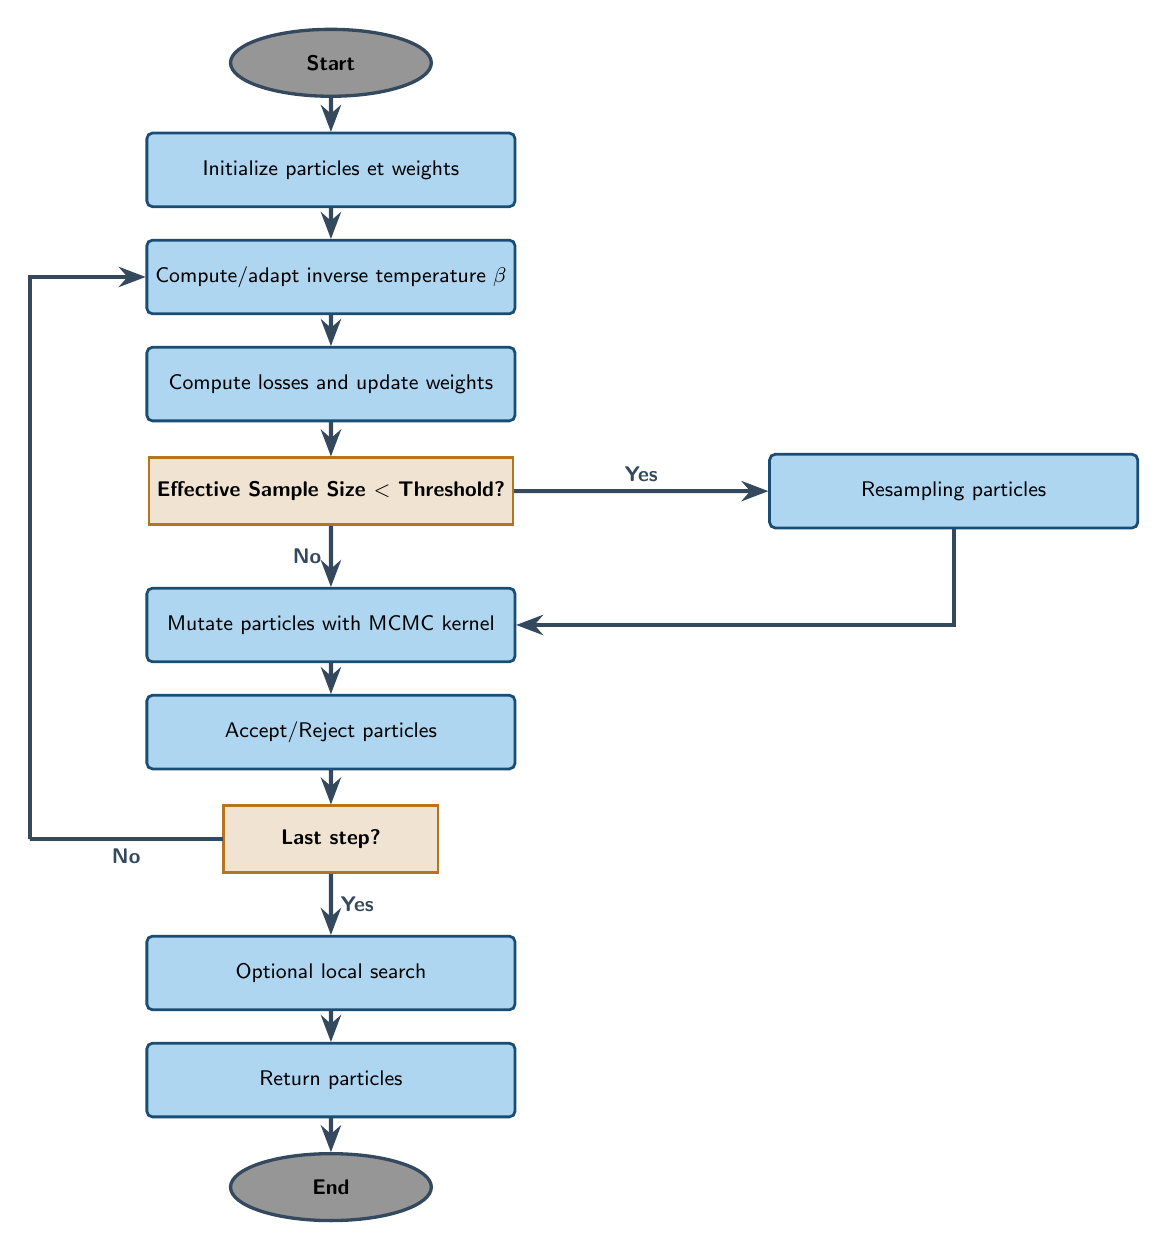
\begin{tikzpicture}[node distance=1.6cm and 0.8cm, scale=0.85, transform shape]
						
						% Nœuds
						\node (start) [startstop] {Start};
						
						\node (init_particles) [process, below of=start] {Initialize particles et weights};
						
						\node (compute_beta) [process, below of=init_particles] {Compute/adapt inverse temperature $\beta$};
						
						\node (weight_update) [process, below of=compute_beta] {Compute losses and update weights};
						
						\node (ess_check) [decision, below of=weight_update] {Effective Sample Size $<$ Threshold?};
						
						\node (resample) [process, right=3.8cm of ess_check] {Resampling particles};
						
						\node (mutation) [process, below of=ess_check, yshift=-0.4cm] {Mutate particles with MCMC kernel};
						
						\node (acceptance) [process, below of=mutation] {Accept/Reject particles};
						
						\node (end_iter) [decision, below of=acceptance] {Last step?};
						
						\node (exploit) [process, below of=end_iter, yshift=-0.4cm] {Optional local search};
						
						\node (output) [process, below of=exploit] {Return particles};
						
						\node (stop) [startstop, below of=output] {End};
						
						% Flèches avec étiquettes améliorées
						\draw [arrow] (start) -- (init_particles);
						\draw [arrow] (init_particles) -- (compute_beta);
						\draw [arrow] (compute_beta) -- (weight_update);
						\draw [arrow] (weight_update) -- (ess_check);
						
						\draw [arrow] (ess_check) -- node[above, arrow_label] {Yes} (resample);
						\draw [arrow] (resample) |- (mutation);
						
						\draw [arrow] (ess_check) -- node[left, arrow_label] {No} (mutation);
						\draw [arrow] (mutation) -- (acceptance);
						\draw [arrow] (acceptance) -- (end_iter);
						
						% Boucle de retour améliorée
						\draw [arrow] (end_iter) -| node[pos=0.25, below, arrow_label] {No} ++(-4.5,0) |- (compute_beta);
						
						\draw [arrow] (end_iter) -- node[right, arrow_label] {Yes} (exploit);
						\draw [arrow] (exploit) -- (output);
						\draw [arrow] (output) -- (stop);
						
					\end{tikzpicture}
				\end{tcolorbox}
			\end{minipage}
			\caption{The flow chart of the Annealed Importance Sampling - Sequential Monte Carlo algorithm}
			\label{ASMCflowchart}
		\end{figure}
		
		To address these challenges, we employ an Annealed Importance Sampling (AIS) combined with Sequential Monte Carlo (SMC) methods. AIS constructs a sequence of intermediate distributions that smoothly transition from an initial, tractable distribution (e.g., a prior over symbolic expressions) to the complex target posterior distribution. This annealing process is guided by a temperature-like parameter that gradually emphasizes the data likelihood, allowing for more efficient exploration of the probability landscape.
		
		SMC enhances this procedure by propagating a population of particles—each representing a candidate symbolic expression—through the sequence of distributions. At each step, particles are reweighted based on the incremental change in the distribution, resampled to focus computational effort on high-probability regions, and mutated via operations. This combination of importance sampling, resampling, and mutation maintains diversity among the particles and prevents premature convergence to suboptimal models.
		
		These features make AIS-SMC particularly well-suited for symbolic regression tasks, where the search space is not only high-dimensional but also structured and discontinuous. 
		
		%\item Then more details: discuss hypotheses to compute the weights, choice of transformations, choice of $\beta$, choice of loss, prior, initial sampling, choice of representation for the polynomials.
		
		Let us now explain in more details how does this procedure goes. The goal is to reconstruct some distribution function $d(z)$, where here $z$ in going to be some polynomial. We will try to reconstruct this density function by series of density function $\pi_n(z_n) = \gamma_n(z_n)/Z_n$ with $n = 1,\dots,N$ is going to be the number of annealing steps, $\pi_n$ is defined in terms of an unnormalized density $\gamma_n$ and we have the normalizing constant $Z_n = \int \gamma_n(z) \mathrm{d}z$. We also assume we have a sequence of inverse temperature constants $\beta_n$, where $0 = \beta_1 < \beta_2 <\dots< \beta_N = 1$. We then define the unnormalized density at level $n$ in terms of a prior distribution $p_0(z)$ over the hypothesis space and a loss function $L(z)$:
		\begin{equation}\label{eq:gamman}
			\gamma_n(z) := d_0(z) \: \exp \left( -\beta_n L(z) \right).
		\end{equation} 
		
		At each epoch, we have a set of particles and weights $\{z_{n-1}^k, w_{n-1}^k\}$ approximating $\pi_{n-1}$ (meaning $\mathbb{E}_{\pi_{n-1}}[f] \approx \frac{\sum_k w_{n-1}^k f(z_{n-1}^k)}{\sum_k w_{n-1}^k}$), and we want to obtain a new set $\{z_n^k, w_n^k\}$ approximating $\pi_n$. To do so, for each particle $z^k_{n-1}$, we propose a new particle $z_n^k \sim q(z_n | z_{n-1}^k)$ and calculate the new unnormalized importance weight $w_n^k$. The latter are updated using the formula 
		\begin{equation}
			w_n^k = w_{n-1}^k \times \alpha_{n}^k
		\end{equation}
		where $\alpha_n^k$ is the incremental importance weight. The standard form for $\alpha_n^k$, which requires introducing an auxiliary backward transition kernel $q(z_{n-1} | z_n)$, is:
		\begin{equation}
			\alpha_n^k = \frac{ \gamma_n(z_n^k) q(z_{n-1}^k | z_n^k) }{ \gamma_{n-1}(z_{n-1}^k) q(z_n^k | z_{n-1}^k) } 
		\end{equation}
		The weights are finally normalized and we get $w_n^k \rightarrow \frac{w_n^k}{\sum_j w_n^j}$.
		
		Let's us now focus on the forward $q(z_n^k | z_{n-1}^k)$ and backward propagation kernel $q(z_{n-1}^k | z_n^k)$ for now. The forward propagation kernel defines how we generate the state at time $n$ given the state at time $n-1$. It gives the probability to transition from $z_{n-1}$ to $z_n$. The backward kernel represents a hypothetical probability of transitioning back from state $z_n$ to state $z_{n-1}$. The purpose of $q$ is to give a proposition for $z_n$ given $z_{n-1}$. For the implementation of the two, we decide to implement an AIS-style MCMC code : we make some move in the space of polynomials, and then accept or reject those new polynomials based on an acceptance rate. So we first need to choose what are the available moves in the space of polynomials. Here are the choices we have made for our symbolic regression task : 
		\begin{itemize}
			\item Coefficient pertubation. Given a polynomial $z_{n-1}$, we choose randomly one of its coefficient and modify it by a random noise from the guassian distribution $\mathcal{N}(0,\sigma^2)$. So for eg : $2 x_1 + 3 x_2^2 \rightarrow  2.1 x_1 + 3 x_2^2$.
			\item Variable multiplication. Given a polynomial $z_{n-1}$, we choose randomly one of his monomial, and multiply it by one of the available variable. So for eg : $2 x_1 + 3 x_2^2 \rightarrow  2 x_1 x_2 + 3 x_2^2$.
			\item Variable division. Given a polynomial $z_{n-1}$, we choose randomly one of his monomial, and divide it by one of its variable. So for eg : $2 x_1 x_2 + 3 x_2^2 \rightarrow  2 x_1 + 3 x_2^2$. 
		\end{itemize}
		The polynomials get mutated at each epoch. The mutation is chosen randomly, assigning probabilities \texttt{p\_{modify}} , \texttt{p\_{multiply}} and \texttt{p\_{divide}} to each possibility. This implementation enables a direct computation of both the forward and backward propagation kernels. In particular, for the case of coefficient perturbations, the transition is symmetric. That is,
		\begin{equation}
			q(z_n^k \mid z_{n-1}^k) = q(z_{n-1}^k \mid z_n^k),
		\end{equation}
		which significantly simplifies the computation of the incremental importance weight.
		
		However, this symmetry does not hold in general. For other types of operations—such as multiplication or division by a variable—the transition from \( z_{n-1}^k \) to \( z_n^k \) is generally not equivalent to the reverse transition from \( z_n^k \) to \( z_{n-1}^k \). In such cases $q(z_n^k \mid z_{n-1}^k) \ne q(z_{n-1}^k \mid z_n^k)$ and particular care must be taken in the computation of the backward propagation kernel.
		
		
		The acceptance ratio for the MCMC algorithm is given by : 
		\begin{equation}\label{eq:acceptanceratio}
			A(z_n,z_{n-1}) = \mathrm{min} \left(1,\frac{ \gamma_n(z_n^k) q(z_{n-1}^k | z_n^k) }{ \gamma_{n-1}(z_{n-1}^k) q(z_n^k | z_{n-1}^k) }  \right)
		\end{equation}
		We then draw $u\sim \mathrm{Uniform}(0,1)$, accept the new particle if $u<A(z_n,z_{n-1})$ and reject it otherwise.

		We have adapted the classic approach outilned above. As can be seen in \eqref{eq:gamman}, what matters the most to determine $\gamma_{n}$ is not the inverse temperature, but rather the product of the inverse temperature and the loss function. Therefore, instead of implementing an arbitrary schedule for $\beta$, we employed an adaptive temperature approach. The number of particles accepted at each run is monitored. We aim at following the following schedule as function of the \texttt{epoch}:
		\begin{equation} \label{eq:acceptanceratioschedule}
			\texttt{acceptance\_ratio} = 0.8 - 0.5 \times \left(\frac{\texttt{epoch}}{\texttt{n\_epochs}}\right),
		\end{equation}
		where \texttt{n\_epochs} is the total number of epochs. If we accept more particle (in the 5 last epochs), we decrease the temperature by 5\%, if we accept less we increase it by 5\%. This encourages exploration during the early stages of training and gradually transitions to a more selective regime. \ce{So we don't use eq.~\eqref{eq:acceptanceratio} at all? This is not clear to me.} 
		
		Before closing the section, we need to discuss what is the Loss function we choose. It is required to compute the unormalized distribution $\gamma_n$. Assume that we have $z = \sum_k c_k X_k$, where $c_k$ are the coefficients of the polynomials, and $X_k$ is a short notations for all the possible monomials up to a given degree (so if we have $x$ and $y$ as variables, and the maximum degree is 2, then $X_k$ are $1, x, y, x^2, y^2, x y$). For the Loss function, we decided to take : 
		\begin{equation} \label{eq:lossreg}
			L(z) = \sum_{i} z(x_i)^2 + \frac{\lambda}{\sum_k |c_k|}
		\end{equation}
		So the first term is just the sum of the squared of the polynomial evaluated on the data. We want to make this 0 so we find polynomial that annihilates our data. The second part is a regularisation factor: it prevents the algorithm to send all the coefficient to 0, which would give a trivial solution to the problem. We typically take $\lambda \sim \mathcal{O}(1000)$.
		
		%\item Analysis after AIS: select the best polynomials and do exploitation on the coefficients (without MC: we keep only the proposal of it betters the polynomial).
		
		Once the Annealing loop is over, we end up with a total of $n_{\rm sample}$ particles, which in principle should be close to annihilate our data, but whose coefficients may need some more fine tuning. To deal with it, we ran a quick exploitation phase, where, for each polynomial, we now only modify its coefficients, with a pertubation $\epsilon \sim \mathcal{N}(0, \sigma_1)$, and keep the new particle, only if the Loss function is now getting smaller. This allow to fine-tune the coefficients. \ce{Mention threshold? And number of iterations?}

%		\bd{Results for naive choices of parameters (numbers of iteration and particles, probabilities, $\beta$) and motivate them (we want some exploration and then exploitation, not too long computations): for multiple runs we find multiple polynomials (good polynomial: after exploitation we convert the coefficients to integers and square roots, and recompute loss without regularisation, select with threshold). Quantify it nicely: success rates for each polynomials, and absolute number of success, failing rate. Total time needed, without cluster or fancy computers.}
	%\end{itemize}
	
\section{Results} \label{sec:results}
	\subsection{Initialisation of the algorithm}
	We initialized the algorithm with \ce{Give $\lambda$? Do we have all parameters here?}
	\begin{equation}	\label{eq:sample10000adaptativetemp}
		\begin{aligned}
			&\texttt{n\_epochs = 1000},\\
			&\texttt{beta  = 1e-6}, \\
			&\texttt{p\_{modify} = 0.5},\\
			&\texttt{p\_{multiply} = 0.25},\\
			&\texttt{p\_{divide} = 0.25}. 
		\end{aligned}
	\end{equation}
	This strategy was determined empirically through trial and error; a systematic analysis of its optimization is left for future work. For the representation of polynomials, we adopt a vectorial approach: each polynomial is represented as an array of its coefficients $\{c_k\}$, where $k \in \{1,\dots,n_{\text{mon}}\}$ and $n_{\text{mon}}$ denotes the number of available monomials, determined by the chosen maximum degree \texttt{max\_degree} and the number of variables. We also impose a constraint on the maximum number of terms within a single polynomial \texttt{max\_num\_monomials} to promote sparsity. An alternative approach would be to encourage sparsity through the prior distribution or within the loss function formulation. For the simulations we have done, we chose : 
	\begin{equation} \label{eq:parampol}
		\begin{aligned}
			&\texttt{max\_degree = 4},\\
			&\texttt{max\_num\_monomials = 6.}
		\end{aligned}
	\end{equation}
	With these parameters and given that we are dealing with $5$ variables, $n_{\text{mon}} = 126$.

	\subsection{Analysis of a typical run}
	After a run, the 1000 particles are typically distributed into less than 10 different type of polynomials. \ce{Check the exact number. Update with a new run.} Each particles of a given type share the same monomials, but their coefficients fluctuate a bit. We select the representative of each type that features the minimal loss (without the regularisation, $\lambda=0$, see eq.~\eqref{eq:lossreg}). Here is an example of output for a given run: \ce{Here $\texttt{threshold} = 0.1$ and $\texttt{steps} = 1000$ for the local search.}
	\begin{subequations}
	    \begin{align}
			1.999\,x_{2} - 1.999\,x_{2}x_{8} + 1.414\,x_{1}x_{10} + 1.999\,x_{1}x_{4} - x_{10}^{2}x_{2}x_{8},\quad &L^{(\lambda = 0)} \simeq 2 \times 10^{-4},  \label{eq:expol1}\\
			2\,x_{2} - 1.999\,x_{2}x_{8} + 1.415\,x_{1}x_{8}x_{10} + 2.001\,x_{1}x_{4}x_{8} - 2.002\,x_{2}x_{4}^{2}x_{8},\quad &L^{(\lambda = 0)} \simeq 3 \times 10^{-3}, \label{eq:expol2}\\
			x_{1}x_{8}x_{10} + 1.416\,x_{1}x_{4}x_{8} - 1.516\,x_{2}x_{4}^{2}x_{8},\quad &L^{(\lambda = 0)} \simeq 3 \times 10^{2}, \label{eq:expol3}\\
			2\,x_{2} - 1.972\,x_{2}x_{8} + 0.816\,x_{1}x_{10} + 1.369\,x_{1}x_{4} - 0.442\,x_{10}^{2}x_{2},\quad &L^{(\lambda = 0)} \simeq 3 \times 10^{2}, \label{eq:expol4}
		\end{align}
	\end{subequations}
	where we normalised the coefficients by setting one of them to $1$ or $2$. Then, we filter out the polynomials with loss higher than $1$, as the polynomials~\eqref{eq:expol3} and~\eqref{eq:expol4}, which do not annihilate the data. Given that the coefficients of the gradient $\nabla V$ are only integers and square roots of integers, the coefficients of the polynomials annihilating $\nabla V$ must be combinations of rational numbers or square roots thereof. We then deduce from eq.~\eqref{eq:expol1} and~\eqref{eq:expol2} the candidate annihilator polynomials for the above example:
	\begin{equation}
		\begin{gathered}
			2\,x_{2} - 2\,x_{2}x_8 + \sqrt{2}\,x_{1}x_{10} + 2\,x_{1}x_{4} - x_{2}x_8x_{10}^{2},\\
	      2\,x_{2} - 2\,x_{2}x_8 + \sqrt{2}\,x_{1}x_8x_{10} + 2\,x_{1}x_{4}x_8
	      		- 2\,x_{2} x_{4}^{2}x_8.
		\end{gathered}
	\end{equation}

	\ce{Change of philosophy here: after SR, we select the best particle, and perform local search. If loss get very low and coefficient not zero, considered as annihilator polynomial. Then filter out the particles containing this polynomial, and repeat on the best particles of the remaining set. Keep it concise. Maybe plot of the loss for the best particle during local search.}

	\subsection{Statistics}
	We performed 1000 independent runs with the same parameters as above, each involving 1000 particles. It takes approximately 600\,s to do a single run without local search on a regular computer. The code finds the 8 different following polynomials: \ce{Sort polynomials in accordance with their frequency.} 
	\begin{subequations} \label{eq:pols}
	 \begin{align}
	   p_{1} &= -\sqrt{2}\,x_{1} + \sqrt{2}\,x_{1}x_8 + x_{2}x_8x_{10} - \sqrt{2}\,x_{2}x_{4}x_8,\\
	   p_{2} &= 2\,x_{2} - 2\,x_{2}x_8 + \sqrt{2}\,x_{1}x_{10} + 2\,x_{1}x_{4} - x_{2}x_8x_{10}^{2},\\
	   p_{4} &= \sqrt{2}\,x_{2} - \sqrt{2}\,x_{2}x_8 + \sqrt{2}\,x_{1}\,x_{4} + x_{1}x_8x_{10}
	   		- x_{2}x_{4}x_8x_{10},\\
	   p_{3} &= 2\,x_{2} - 2\,x_{2}x_8 + \sqrt{2}\,x_{1}x_8x_{10} + 2\,x_{1}x_{4}x_8
	   		- 2\,x_{2} x_{4}^{2}x_8,\\
	   p_{7} &= -\sqrt{2}\,x_{1}^{2}x_{4} + \sqrt{2}\,x_{2}^{2}x_{4} + \sqrt{2}\,x_{1}x_{2}x_{4}^{2} - x_{1}^{2}x_{10}
	   		- x_{2}^{2}x_{10}, \\
	   p_{5} &= -2\,x_{1} - 2\,x_{2}x_{4}- 2\,x_{1}x_{4}^{2} + 2\,x_{1}x_8 + \sqrt{2}\,x_{2}x_{10}
	   		+ x_{1}x_8x_{10}^{2},\\
	   p_{8} &= -2 + 4\,x_{8} - 2\,x_8^2 + 2\,x_{4}^2 x_8 - x_8^2 x_{10}^2,\\
	   p_{6} &= -2\,x_{2}x_{4} - 2\,x_{1}x_{4}^{2} + 2\,x_{2}x_{4}x_8 + \sqrt{2}\,x_{2}x_{10} 
	   		- \sqrt{2}\,x_{2}x_8x_{10} +  x_{1}x_8x_{10}^{2},
	 \end{align}
	\end{subequations}
	where $x_{8} = e^{\tilde{x}_{8}}$. They are found with different frequencies, with some polynomials occurring more often than others, as reported in tab.~\ref{table:results}. The algorithm typically identifies an average of $2.2$ distinct polynomials per run, with a maximum number of $4$, demonstrating its capacity to uncover multiple solutions simultaneously. The algorithm failed at finding a solution in only 3 runs. This is summed up in fig.~\ref{fig:piechart}. Note that in $77\%$ of the time the algorithm finds more than a single solution, demonstrating the robustness of the method.

	\begin{table}
		\centering
		\renewcommand{\arraystretch}{1.3}
		\begin{tabular}{c|ccccccccc}
			& $p_{1}$ & $p_{2}$ & $p_{4}$ & $p_{3}$ & $p_{7}$ & $p_{5}$ & $p_{8}$  & $p_{6}$&  $\varnothing$  \\\hline\hline
			Frequency & 92.6\% & 75.0\% & 51.9\% & 1.7\% & 0.2\% & 0.7\% & 0.7\% & 0.3\% & 0.1\% \\
			Maximum \# of representatives & 1000 & 1000 & 991 & 869 & 879 & 710 & 207 & 18 & --
		\end{tabular}
		\caption{Statistics of the ability of the ASMC algorithm to produce the polynomials~\eqref{eq:pols} on 1000 runs with parameters~\eqref{eq:sample10000adaptativetemp} and~\eqref{eq:parampol}. The frequencies represent the percentage of runs featuring a given polynomial in its outputs, and the maximum number of representatives gives the maximum number of particles representing the polynomial in a given run. The column $\varnothing$ counts the runs that failed to produce an annihilator polynomial.}
		\label{table:results}
	\end{table}

	\begin{figure}
		\centering
		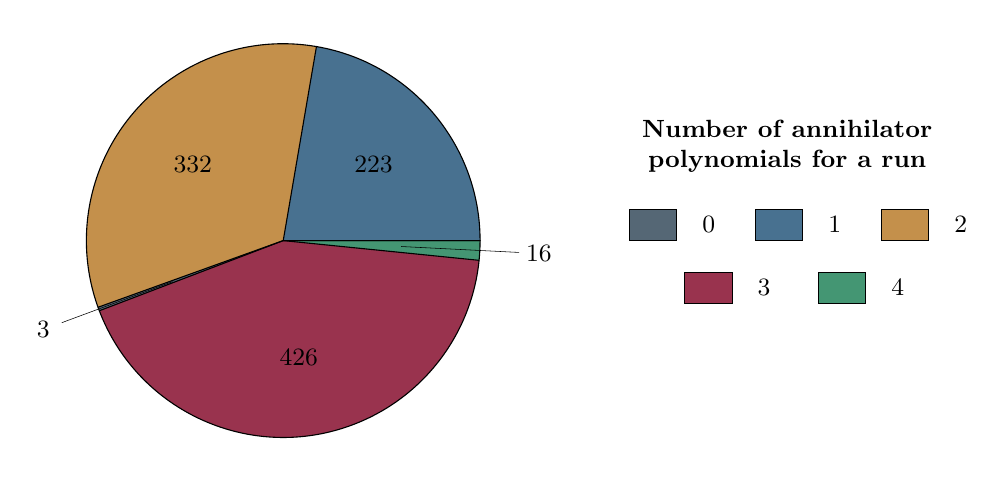
\begin{tikzpicture}[scale=2]

\def\radius{1.25}

\fill[myblue!80] (0:0) -- (0:\radius) arc [start angle=0,end angle={360*0.223},radius=\radius] -- (0:0);
\draw ({360*0.223/2:0.6*\radius})node [black] {\small 223};

\fill[myorange!80] (0:0) -- ({360*0.223}:\radius) arc [start angle={360*0.223},end angle={360*(0.223+0.332)}, radius = \radius] -- (0:0);
\draw ({360*(0.223+0.332/2)}:0.6*\radius) node [black] {\small 332};

\fill[myblack!80] (0:0) -- ({360*(0.223+0.332)}:\radius) arc [start angle={360*(0.223+0.332)},end angle={360*(0.223+0.332+0.003)},radius = \radius] -- (0:0);
\draw [very thin] ({360*(0.223+0.332+0.003/2)}:{\radius*0.6}) -- ({360*(0.223+0.332+0.003/2)}:\radius*1.2);
\draw ({360*(0.223+0.332+0.003/2)}:\radius*1.3) node {\small 3};  

\fill[myred!80] (0:0) -- ({360*(0.223+0.332+0.003)}:\radius) arc [start angle={360*(0.223+0.332+0.003)},end angle={360*(0.223+0.332+0.003+0.426)},radius = \radius] -- (0:0);
\draw ({360*(0.223+0.332+0.003+0.426/2)}:0.6*\radius) node [black] {\small 426};

\fill[mygreen!80] (0:0) -- ({360*(0.223+0.332+0.003+0.426)}:\radius) arc [start angle={360*(0.223+0.332+0.003+0.426)},end angle={360*(0.223+0.332+0.003+0.426+0.016)},radius = \radius] -- (0:0);
\draw [very thin] ({360*(0.223+0.332+0.003+0.426+0.016/2)}:\radius*0.6) -- ({360*(0.223+0.332+0.003+0.426+0.016/2)}:\radius*1.2);
\draw ({360*(0.223+0.332+0.003+0.426+0.016/2)}:\radius*1.3) node {\small 16};  


\draw (0:0) -- (0:\radius) arc [start angle=0,end angle={360*0.223}, radius = \radius] -- (0:0);
\draw ({360*0.223}:\radius) arc [start angle={360*0.223},end angle={360*(0.223+0.332)}, radius = \radius] -- (0:0);
\draw ({360*(0.223+0.332)}:\radius) arc [start angle={360*(0.223+0.332)},end angle={360*(0.223+0.332+0.003)}, radius = \radius] -- (0:0);
\draw ({360*(0.223+0.332+0.003)}:\radius) arc [start angle={360*(0.223+0.332+0.003)},end angle={360*(0.223+0.332+0.003+0.426)},radius = \radius] -- (0:0);
\draw ({360*(0.223+0.332+0.003+0.426)}:\radius) arc [start angle={360*(0.223+0.332+0.003+0.426)},end angle={360*(0.223+0.332+0.003+0.426+0.016)}, radius = \radius] -- (0:0);



\draw (3.2,0.6) node [align=center, font= \bfseries\small] {Number of annihilator\\polynomials for a run};
\draw[black, fill=myblack!80] (2.2,0) rectangle +(0.3,0.2);
\draw (2.6,0.1) node [right] {\small $0$};
\draw[black, fill=myblue!80] (3,0) rectangle +(0.3,0.2);
\draw (3.4,0.1) node [right] {\small $1$};
\draw[black, fill=myorange!80] (3.8,0) rectangle +(0.3,0.2);
\draw (4.2,0.1) node [right] {\small $2$};
\draw[black, fill=myred!80] (2.55,-0.4) rectangle +(0.3,0.2);
\draw (2.95,-0.3) node [right] {\small $3$};
\draw[black, fill=mygreen!80] (3.4,-0.4) rectangle +(0.3,0.2);
\draw (3.8,-0.3) node [right] {\small $4$};
 
\end{tikzpicture}
		\caption{Pie chart of the repartition of the number of distinct polynomials found in a single run.}
		\label{fig:piechart}
	\end{figure}
	  
	We have tracked the appearance of the polynomials~\eqref{eq:pols} during each of the 1000 runs. To do so, we have counted at each epoch the number of particles including the same monomials as the annihilator polynomials.\footnote{Thus, a particle featuring the same monomials as one of the polynomials~\eqref{eq:pols} will be counted, even if the coefficients do not match, and if there are additional monomials.} The total number of particles reproducing at least one of the annihilator polynomials listed in eq.~\eqref{eq:pols} is plotted in fig.~\ref{fig:count_pol_all_beta}, together with the evolution of the inverse temperature $\beta$, both averaged on the 1000 runs. The proportion of annihilator polynomials among the particles start to be significant after approximately 700 epochs. It then increases quickly and, towards the end of each run, an average of $88\%$ of the particles do reproduce one of the annihilator polynomials, with a standard deviation of $20\%$. The evolution of this proportion is explained by the structure of the method: the code favours the particles with highest weights, and thus those that cause a significant improvement to the loss function, at each resampling. Once an annihilator polynomials is reached, it colonises larger and larger proportions of the particles at each resampling.

	The evolution of the inverse temperature is dictated by eq.~\eqref{eq:acceptanceratioschedule}. Note that $\beta$ is equal to $0.02$ in average at the end of the runs. The temperature is thus still quite high, which favours diversity. This is a key ingredient to get more than one candidate polynomials per run. The end value of $\beta$ is intimately linked to the choice of target acceptance ratio in eq.~\eqref{eq:acceptanceratioschedule}: the lower the acceptance ratio, the higher the inverse temperature $\beta$. On the one hand, if the ratio is too low, very few particles get mutated and it's difficult to explore the space of polynomials and to have diverse outputs. On the other hand, if the ratio is too high, there are too many mutations: the output features a large number of polynomials, but lots of them do not converge to an annihilator polynomials because the algorithm is not selective enough. It is a matter of balance between exploration and exploitation.

	The dynamics of appearance of each annihilator polynomial is plotted in fig.~\ref{fig:count_pol_indiv}, averaged on the 1000 runs. The dynamics depend strongly on the polynomial and we observe three different classes. In the first case, for $p_{1}, p_{2}$ and $p_{4}$, the first occurrences appear typically after only few dozen of epochs; and in the the second one, constituted of $p_{3}, p_{5}, p_{7}$ and $p_{8}$, after few hundreds of epochs. The last class has $p_{6}$ as its only representative. This polynomial is very difficult to produce, and when it appears it is only towards the end of the runs. The stair-step patterns, with sudden jumps in the population of the polynomials alternating with phases of stagnation, are due to the use of resampling in the algorithm. When a particle get close enough to an annihilating polynomials, its loss gets lowered significantly faster than the one of the other particles. This induces an increase of its weight and it will populate a large part of the sample at the next resampling. The coefficients get improved during the stagnation phases, inducing an increase of the polynomials weights, and thus even larger colonizations during the following resamplings. This also induces a competition between the annihilator polynomials, the ones that get bettered the more easily (typically those with fewest terms) are favoured. This mechanism explains the decrease in the averaged population of the polynomial $p_{8}$ observed after 800 epochs in fig.~\ref{fig:count_pol_indiv}.

	The best loss for each of the 1000 runs is shown in fig.~\ref{fig:lossallASMC} in blue, together with their mean value in yellow, with a logarithmic $y$-axis. The losses here do include the regularisation factor $\lambda$, see eq.~\eqref{eq:lossreg}. For a given run, we are plotting the best loss at each epoch, the curves thus do not follow single particles. On average the loss get bettered by two orders of magnitude during a run, illustrating the convergence of the algorithm. \ce{Discuss the fact that it's still high. Also linked to the low $\beta$. Sufficient to distinguish good polynomials using local search.}

	\begin{figure}
		\centering
		\subfigure{ \label{fig:count_pol_all_beta}
			\begin{tikzpicture}
		  		\draw (0,0) node (fig1) {\includegraphics[scale=0.7]{Figures/Count_pol_all_beta_1000runs_13.pdf}};
		  		\draw ($(fig1.north west) + (0,0)$) node {\small (a)};
		  		\draw (8.25,0) node (fig2) {\includegraphics[scale=0.7]{Figures/Count_pol_indiv_1000runs_13.pdf.pdf}};
		  		\draw ($(fig2.north west) + (0,0)$) node {\small (b)};
		  	\end{tikzpicture}
		}
		\subfigure{\label{fig:count_pol_indiv}}
		\vspace{-1cm}
		\caption{(a) Evolution of the mean number of particles reproducing a target polynomial, along with its $1\sigma$ deviation, for the parameters described in~\eqref{eq:sample10000adaptativetemp} (left scale) and evolution of the inverse temperature $\beta$ and its $1\sigma$ deviation (right scale). (b) Dynamics of the mean number of particles reproducing each polynomial in eq.~\eqref{eq:pols} (the scale of the $y$-axis is logarithmic).}
		\label{fig:evolutionoftargetreproduction}
	\end{figure}

	\begin{figure}[h!]
		\centering
		\includegraphics[scale=0.75]{Figures/Loss_all_ASMC_1000runs_13.pdf}
		\caption{Evolution of the lowest loss during each of the 1000 runs (in blue) and their average (in yellow). The losses are computed with the regularisation factor $\lambda$, see eq.~\eqref{eq:lossreg}.}
		\label{fig:lossallASMC}
	\end{figure}

	\subsection{Supergravity solution}
	In the previous section, we introduced a numerical method that enabled symbolic regression, yielding a set of polynomials that vanish on our dataset, as presented in eq.~\eqref{eq:pols}. We know from sec.~\ref{sec:gadientlocalanalysis} that the manifold we are aiming at parametrising is three-dimensional. As the parameter space is of dimension $5$, we only need two constraints to define the solutions, and the eight polynomials of eq.~\eqref{eq:pols} are not independent. We are however only interested in finding an analytic parametrisation of the solutions manifold, and the easiest to find it is to solve the system
	\begin{equation}\label{eq:solvepol}
		p_i = 0, \quad \forall i \in {1,\dots,8}.
	\end{equation}
	This leads to the following rules between the parameters:
	\begin{equation}\label{eq:rulex8x10}
		\begin{cases}
			\displaystyle e^{\tilde{x}_{8}} = \frac{x_{1}^{2}+x_{2}^{2}}{x_{2}^{2} + \big(x_{1}-x_{2}x_{4}\big)^{2}},\\[10pt]
			\displaystyle x_{10} = \sqrt{2}\,x_{4}\,\frac{x_{2}^{2} - x_{1}^{2}+x_{1}x_{2}x_{4}}{x_{1}^{2}+x_{2}^{2}}.
		\end{cases}
	\end{equation}
	Alternatively, the system can be recast as:
	\begin{equation}
		\begin{cases}
			\displaystyle x_{1} = \frac{x_{2}}{e^{\tilde{x}_{8}}-1}\,\Big(x_{4}\,e^{\tilde{x}_{8}} \pm \sqrt{-1+\big(2+x_{4}^{2}\big)\,e^{x_{8}}-e^{2\tilde{x}_{8}}}\Big),\\[8pt]
			\displaystyle x_{10} = \mp\,e^{-\tilde{x}_{8}}\,\sqrt{-2+2\,\big(2+x_{4}^{2}\big)\,e^{\tilde{x}_{8}}-2\,e^{2\tilde{x}_{8}}},
		\end{cases}
	\end{equation}
	or
	\begin{equation}
		\begin{cases}
			\displaystyle x_{1} = \frac{x_{2}}{\sqrt{2}}\,\frac{e^{\tilde{x}_{8}/2}}{e^{\tilde{x}_{8}}-1}\,\Big(-x_{10}\,e^{\tilde{x}_{8}/2} \pm \sqrt{2-4\,e^{\tilde{x}_{8}}+e^{2\tilde{x}_{8}}\big(2+x_{10}^{2}\big)}\Big),\\[8pt]
			\displaystyle x_{4} = \pm \frac{e^{-x_{8}/2}}{\sqrt{2}}\,\sqrt{2-4\,e^{\tilde{x}_{8}}+e^{2\tilde{x}_{8}}\big(2+x_{10}^{2}\big)}.
		\end{cases}
	\end{equation}
	As anticipated, this defines a three-parameter manifold. We tested analytically that $\nabla V = 0$ for any of these rules. The three-parameter manifold then corresponds defines a three-dimensional space of flat directions of the half-maximal supergravity scalar potential.\footnote{One might argue that only two of the eight polynomials are sufficient to fully characterize the solution. That is, choosing any pair $(i,j) \in {1, \dots, 8}$ may suffice to extract a complete description. In practice, this is not entirely accurate. While such a pair can yield partial constraints -- for example, recovering eq.~\eqref{eq:rulex8x10} -- it may also produce alternative (and potentially less general) parameterisations. Upon inspection, all such partial rules are found to be consistent with, and included in, the most general expressions given in eq.~\eqref{eq:rulex8x10}.}

	The supergravity solution can be shown to preserve a ${\rm U}(1)\times{\rm U}(1)$ gauged symmetry. Using the parametrisation~\eqref{eq:rulex8x10}, the $(x_{1},x_{2},x_{4})$ moduli space is most nicely parametrised using the change of coordinates
	\begin{equation}
		x_{1} = r\cos(\theta)\cos(\Phi), \quad x_{2} = r\cos(\theta)\sin(\Phi) \quad {\rm and} \quad x_{4} = r\sin(\theta),
	\end{equation}
	for which the Zamolodchikov metric reads
	\begin{equation}
		\d^{2}s_{\rm Zam.} = -\,\d r^{2} - r^{2}\,\bigg(\d \theta^{2} - r\cos(\theta)\,\d \theta\d\Phi + \sin(\theta)\,\d r\d\Phi + \frac{1}{2}\,\big(3+r^{2}-\cos(2\theta)\big)\,\d\Phi^{2} \bigg).
	\end{equation}

\section{Conclusion}

In this work, we have presented a novel machine learning approach to systematically identify and characterize flat directions in supergravity scalar potentials. Our methodology combines gradient descent sampling with annealed importance sampling for symbolic regression, demonstrating its effectiveness on a 5-scalar subsector of 3d (1,1) supergravity derived from 
$AdS_3 \times S^3 \times T^4$ compactifications of IIB supergravity.

We developed a robust pipeline that transitions from numerical exploration to analytical understanding. The gradient descent procedure successfully samples the flat direction manifold, while local PCA analysis reveals its intrinsic dimensionality. Most notably, our annealed importance sampling approach to symbolic regression automatically discovers polynomial constraints characterizing the manifold, bypassing the computational complexity that renders direct symbolic manipulation intractable.

Our analysis reveals that the 5-dimensional scalar space contains a 3-dimensional conformal manifold, with one direction potentially gauge-fixable. The discovered solution preserves $U(1) \times U(1)$ gauged symmetry and exhibits a rich spectrum structure. The Zamolodchikov metric on the moduli space, parametrized by spherical-like coordinates, provides a concrete geometric description of the conformal manifold.

The method demonstrates remarkable efficiency and reliability. The algorithm discovers eight distinct polynomial relations with varying frequencies, suggesting a hierarchical structure in constraint discovery. Futhermore, upon 1000 the algorithm failed at finding any solution in only 3 cases, demonstrating the robustness of the method. 

This approach opens several promising avenues for advancement. The scalability to higher-dimensional cases represents the most immediate challenge and opportunity. By increasing the number of particles, refining the annealing schedule, and optimizing polynomial search strategies, we anticipate extending this methodology to the full 13-scalar theory and potentially to other supergravity models. 

Beyond technical improvements, this work suggests a broader paradigm for exctrating conformal manifolds in string theory and supergravity. This analytical constraints from numerical data could prove invaluable for classifying flat directions across different theories, understanding moduli stabilization mechanisms, and exploring the landscape of consistent supergravity backgrounds.

The marriage of machine learning techniques with traditional supergravity analysis represents a step toward more systematic approaches to understanding the rich geometric structures underlying these theories. As computational power increases and algorithms improve, we envision this methodology becoming a standard tool for exploring the intricate relationships between geometry, symmetry, and dynamics in supergravity theories.

While the specific solution found in this 5-scalar model may have limited direct physical applications, the demonstrated feasibility of our approach and its potential for systematic classification of flat directions across the supergravity landscape make it a valuable addition to the theoretical physicist's toolkit.

\appendix
\section{Comparison with AIFeynman} \ce{Appendix?}
In comparaison with state of the art technique, we have used the AIFeynman algorithm on our data set, with again $x_8 = \exp(\tilde{x}_8)$, such that we again look for polynomial expressions. We have run it with the following configuration 
\begin{equation}
	\begin{aligned}
		&\texttt{BF\_try\_time} = 300, \\
		&\texttt{polyfit\_deg} = 6, \\
		&\texttt{NN\_epochs} = 5000.\\
	\end{aligned}
\end{equation}
The first parameter fixes the time limit in seconds for each brute force call, \texttt{polyfit\_deg} gives the maximum degree of the polynomial tried by the polynomial fit routine and \texttt{NN\_epochs} is the number of training epoch for the internal neural network. The function used for the brut force tests are 
\begin{equation}
\texttt{+*-/><} \sim \texttt{\textbackslash R1}
\end{equation}
The binary operations are addition, multiplication, substraction and division. The unary ones are inverse, increment, decrement, negation and square root. Finally there is a nonary one, the unity. For more details we refer to \cite{Udrescu:2019mnk}.

In this algorithm, one tries to fit one of the variables in term of the others. Here, we used it to fit $x_{10}$ in terms of the others. The AIFeynman algorithm finds a solution in TIME : 
\begin{equation}
	\texttt{x\_10 = 1.414213551821*(x\_4-((x\_1/x\_2)-((x\_1/x\_2)/x\_8))}
\end{equation}
which after identifying the numerical factor with $\sqrt 2$ and inverting the relation gives 
\begin{equation}
	- \sqrt 2 x_1 + \sqrt 2 x_1 x_8 + x_2 x_8  x_{10} -\sqrt 2 x_2 x_4 x_8 = 0
\end{equation}
which corresponds to $p_1$ of Eq. \eqref{eq:pols}. While the AIFeynman code is able to recover one of the constraints, it exhibits several drawbacks compared to our method. First, it is significantly slower: it required TIME (to be specified) compared to approximately 600 seconds for a single run of our ASMC algorithm. Moreover, the AIFeynman framework is based on expressing one variable as a function of the others, which assumes the invertibility of the underlying relation. In general, this is not guaranteed for the class of polynomials in Eq. \eqref{eq:pols}, and obtaining a closed-form inverse can be nontrivial or even impossible for higher-degree expressions. In our case, each polynomial involves at most quadratic terms in any single variable, ensuring invertibility, but this property would not hold for more complex models. In addition, AIFeynman is limited to recovering one constraint per run, whereas our ASMC method can discover multiple constraints simultaneously. This is reflected in our results, where each run identified an average of 2.15 polynomials, with up to 4 found in the best case. Finally, the brute-force regression strategy used by AIFeynman makes it less effective for identifying higher-degree polynomials, whose complexity increases the search difficulty. In contrast, our method treats all polynomials as equally probable, regardless of their degree, enabling it to uncover more intricate structures more efficiently \footnote{Note that we do not claim that we have used the AIFeynman in the most optimal way.}.
\newpage
\section{Details on the algorithm}

\begin{algorithm}
	\caption{Local Dimension Estimation using PCA}
	\label{alg:local-dim}
	\begin{algorithmic}[1]
		
		\State \textbf{Function} \textsc{LocalDim1Point}($\texttt{x}$, $\texttt{var\_thres}$)
		\State \hspace{0.5cm} Apply PCA to data matrix $\texttt{x}$
		\State \hspace{0.5cm} Compute explained variance ratios: $\texttt{lambda\_1, lambda\_2,} \ldots, \texttt{lambda\_d}$
		\State \hspace{0.5cm} Compute cumulative variance: $\texttt{cumvar\_k} = \sum_{\texttt{i=1}}^\texttt{k} \texttt{lambda\_i}$ for $\texttt{k = 1, }\ldots\texttt{, d}$
		\State \hspace{0.5cm} Find $\texttt{dim = min\{k : cumvar\_k} \geq \texttt{var\_thres\}}$
		\State \hspace{0.5cm} \textbf{return} $\texttt{dim}$
		\State
		
%		\State \textbf{Function} \textsc{ComputeLocalDim}(\texttt{i, data, neighbors\_idx, var\_thres})
%		\State \hspace{0.5cm} Extract local neighbors : \texttt{local\_neighbors} $\leftarrow$ \texttt{data[neighbors\_idx[i]]}
%		\State \hspace{0.5cm} \texttt{dim} $\leftarrow$ \textsc{LocalDim1Point}(\texttt{local\_neighbors, var\_thres})
%		\State \hspace{0.5cm} \textbf{return} \texttt{[dim, i]}
%		\State

%		\Require \texttt{data} (input data matrix of size \texttt{n $\times$ d}), \texttt{n\_neig} (number of neighbors), \texttt{var\_thres} (variance threshold)
%		\Ensure Local dimensions for all points

		\State \textbf{Function} \textsc{LocalDimNPoints}(\texttt{data, n\_neig, var\_thres})
		\State \hspace{0.5cm} \texttt{n\_points} $\leftarrow$ number of rows in \texttt{data}
		\State \hspace{0.5cm} Initialize \texttt{results} $\leftarrow \emptyset$
%		\State \hspace{0.5cm} Fit KD-Tree on \texttt{data} with \texttt{n\_neig} neighbors \Comment{Find k-nearest neighbors using KD-Tree}
		\State \hspace{0.5cm} Compute \texttt{neighbors\_idx} for all points in \texttt{data}
		\For{\texttt{i = 1} to \texttt{n\_points}} \Comment{Compute local dimensions for all points}
		\State \texttt{result\_i} $\leftarrow$ \textsc{ComputeLocalDim}(\texttt{i, data, neighbors\_idx, var\_thres})
		\State Append \texttt{result\_i} to \texttt{results}
		\EndFor

		
		\Return \texttt{results}
	\end{algorithmic}
\end{algorithm}


In this appendix, we detail the different algorithm that we used. We first here provide a pseudo-code for the AIS-SMC algorithm : 

%\begin{algorithm}
%	\caption{Annealing Importance Sampling for Polynomial Discovery}
%	\label{alg:annealing-is}
%	\begin{algorithmic}[1]
%		\Require $n\_iter$ (number of iterations), $n\_particles$ (number of particles), $target\_acc\_rate(\cdot,\cdot)$ (target acceptance rate), $adaptation\_strength$ (temperature adaptation parameter)
%		
%		\State Initialize particles $\{z_0^{(k)}\}_{k=1}^{n\_particles}$ with sparse polynomials
%		\State Set $w_0^{(k)} = 1/n\_particles$ and $\tilde{w}_0^{(k)} = 1$ for all $k$ \Comment{normalized and unnormalized weights}
%
%		\State $z_{prev} \leftarrow z_0$, $best\_loss \leftarrow \infty$, $acceptance\_history \leftarrow \emptyset$, $q_{ratio}^{(k)}=1$ for all $k$ \Comment{q is the proposal ratio}, $\beta_0 \leftarrow 10^{-8}$
%		
%		\For{$i = 1$ to $n\_iter$} \Comment{Temperature adaptation}
%
%		\State $\beta_{prev} \leftarrow \beta_{current}$, $avg\_acc \leftarrow$ mean$(acceptance\_history)$ \Comment{only of the last 5 epochs}
%		\If{$avg\_acc < target\_acc\_rate(i, n\_iter) - 0.05$}
%		\State $\beta_{current} \leftarrow \beta_{current} \times (1 - adaptation\_strength)$
%		\ElsIf{$avg\_acc > target\_acc\_rate(i, n\_iter) + 0.05$}
%		\State $\beta_{current} \leftarrow \beta_{current} \times (1 + adaptation\_strength)$
%		\EndIf
%
%		
%		\For{$k = 1$ to $n\_particles$} \Comment{Reweighting step}
%		\State Compute $\log \gamma_i(z_i^{(k)}) = -\beta_{current} \times loss(z_i^{(k)}) $
%		\State Compute $\log \gamma_{i-1}(z_{i-1}^{(k)}) = -\beta_{prev} \times loss(z_{prev}^{(k)})$
%		\State $\Delta \log w_i^{(k)} \leftarrow \log \gamma_i(z_i^{(k)}) - \log \gamma_{i-1}(z_{i-1}^{(k)}) + \log q_{ratio}^{(k)}$
%		\EndFor
%		
%		\State Update unnormalized weights: $\tilde{w}_i^{(k)} \leftarrow \tilde{w}_{i-1}^{(k)} \times \exp(\Delta \log w_i^{(k)})$
%		\State Normalize weights: $w_i^{(k)} \leftarrow \tilde{w}_i^{(k)} / \sum_{j=1}^{n\_particles} \tilde{w}_i^{(j)}$
%		\State Compute ESS: $ESS = 1 / \sum_{k=1}^{n\_particles} (w_i^{(k)})^2$
%		
%		\If{$ESS < n\_particles / 2$} \Comment{Resampling}
%		\State Resample particles: $\{z_i^{(k)}\}_{k=1}^{n\_particles} \sim Multinomial(n\_particles, \{w_i^{(k)}\}_{k=1}^{n\_particles})$
%		\State Reset weights: $w_i^{(k)} = 1/n\_particles$, $\tilde{w}_i^{(k)} = 1$ for all $k$
%		\State Update $z_{prev}$ accordingly
%		\EndIf
%		
%		\State $z_{before\_mutation} \leftarrow z_i$ (save current particles)
%
%		\For{$k = 1$ to $n\_particles$} \Comment{Mutating with Metropolis-Hasting}
%		\State Propose $z'^{(k)} \sim q(z'^{(k)} | z_i^{(k)})$ using specialized MH proposal
%		\State Compute $\log p_{current}^{(k)} = -\beta_{current} \times loss(z_i^{(k)}) + sparsity\_prior(z_i^{(k)})$
%		\State Compute $\log p_{proposed}^{(k)} = -\beta_{current} \times loss(z'^{(k)}) + sparsity\_prior(z'^{(k)})$
%		\State $\log \alpha^{(k)} \leftarrow \log p_{proposed}^{(k)} - \log p_{current}^{(k)} + \log q_{ratio}^{(k)}$
%		\State Generate $u^{(k)} \sim \mathcal{U}(0,1)$
%		\If{$\log u^{(k)} < \log \alpha^{(k)}$}
%		\State $z_i^{(k)} \leftarrow z'^{(k)}$ (accept proposal)
%		\EndIf
%		\EndFor
%		
%		\State $acceptance\_rate \leftarrow$ fraction of accepted proposals
%		\State Add $acceptance\_rate$ to $acceptance\_history$
%		\State $z_{prev} \leftarrow z_{before\_mutation}$ (update for next iteration)
%		
%		\EndFor
%
%		
%		\Return final particles, final losses, final weights
%	\end{algorithmic}
%\end{algorithm}

\begin{algorithm}
	\caption{Annealing Importance Sampling for Polynomial Discovery}
	\label{alg:annealing-is}
	\begin{algorithmic}[1]
		\Require \texttt{n\_iter} (number of iterations), \texttt{n\_particles} (number of particles), \texttt{target\_acc\_rate}$(\cdot,\cdot)$ (target acceptance rate), \texttt{adaptation\_strength} (temperature adaptation parameter)
		
		\State Initialize particles $\{\texttt{z\_0}^{(k)}\}_{k=1}^{\texttt{n\_particles}}$ with sparse polynomials
		\State Set $\texttt{w\_0}^{\texttt{(k)}} = 1/\texttt{n\_particles}$ and $\texttt{w\_unorm\_0}^{\texttt{(k)}} = 1$ for all $\texttt k$ \Comment{normalized and unnormalized weights}
		\State $\texttt{z\_prev} \leftarrow \texttt{z\_0}$, $\texttt{best\_loss} \leftarrow \infty$, $\texttt{acceptance\_history} \leftarrow \emptyset$, $\texttt{q\_ratio}^{\texttt{(k)}}=1$ for all $k$, $\texttt{beta\_0} \leftarrow \texttt{init\_beta}$ \Comment{q is the proposal ratio}
		
		\For{$\texttt{i = 1}$ to \texttt{n\_iter}} \Comment{Temperature adaptation}
		\State $\texttt{beta\_{prev}} \leftarrow \texttt{beta\_current}$
		\State $\texttt{avg\_acc} \leftarrow$ mean$(\texttt{acceptance\_history})$ \Comment{only of the last 5 epochs}
		\If{$\texttt{avg\_acc < target\_acc\_rate(i, n\_iter) - 0.05}$}
		\State $\texttt{beta\_current} \leftarrow \texttt{beta\_current} \times \texttt{(1 - adaptation\_strength)}$
		\ElsIf{$\texttt{avg\_acc > target\_acc\_rate(i, n\_iter) + 0.05}$}
		\State $\texttt{beta\_current} \leftarrow \texttt{beta\_current} \times \texttt{(1 + adaptation\_strength)}$
		\EndIf
		
		\For{$\texttt{k = 1}$ to \texttt{n\_particles}} \Comment{Reweighting step}
		\State Compute $\texttt{log(gamma\_i(z\_i}^{\texttt{(k)}} \texttt{)) = - beta\_current} \times \texttt{loss}(\texttt{z\_i}^{\texttt{(k)}}) $
		\State Compute $\texttt{log(gamma\_(i-1)}(\texttt{z\_(i-1)}^{\texttt{(k)}}\texttt{)) = - beta\_prev} \times \texttt{loss}(\texttt{z\_prev}^{\texttt{(k)}})$
		\State $\Delta \log \texttt{w\_i}^{\texttt{(k)}} \leftarrow \texttt{log(gamma\_i(\texttt{z\_i}}^{\texttt{(k)}}  \texttt{) - log(gamma\_(i-1)(z\_(i-1)}^{\texttt{(k)}} \texttt{) + log(q\_ratio}^{\texttt{(k)}}\texttt)$
		\EndFor
		
		\State Update unnormalized weights: $\texttt{w\_unorm\_i}^{\texttt{(k)}} \leftarrow \texttt{w\_unorm\_(i-1)}^{\texttt{(k)}} \times \texttt{exp(}\Delta \texttt{log w\_i}^{\texttt{(k)}}\texttt)$
		\State Normalize weights: $\texttt{w\_i}^{\texttt{(k)}} \leftarrow \texttt{w\_unorm\_i}^{\texttt{(k)}} \texttt/ \sum_{\texttt{j=1}}^{\texttt{n\_particles}} \texttt{w\_unorm\_i}^{\texttt{(j)}}$
		\State Compute ESS: $\texttt{ESS = 1 /} \sum_{\texttt{k=1}}^{\texttt{n\_particles}} \texttt{(w\_i}^{\texttt{(k)}})^\texttt2$
		
		\If{$\texttt{ESS < n\_particles / 2}$} \Comment{Resampling}
		\State Resample particles: $\{\texttt{z\_i}^{\texttt{(k)}}\}_{\texttt{k=1}}^{\texttt{n\_particles}} \sim \texttt{Multinomial}(\texttt{n\_particles}, \{\texttt{w\_i}^{\texttt{(k)}}\}_{\texttt{k=1}}^{\texttt{n\_particles}})$
		\State Reset weights: $\texttt{w\_i}^{\texttt{(k)}} = \texttt{1/n\_particles}$, $\texttt{w\_unorm\_i}^{\texttt{(k)}} \texttt{= 1}$ for all $\texttt k$
		\State Update $\texttt{z\_prev}$ accordingly
		\EndIf
		
		\State $\texttt{z\_before\_mutation} \leftarrow \texttt{z\_i}$ (save current particles)
		\For{$\texttt{k = 1}$ to \texttt{n\_particles}} \Comment{Mutating with Metropolis-Hasting}
		\State Propose $\texttt{z}'^{\texttt{(k)}} \sim \texttt{q}(\texttt{z}'^{\texttt{(k)}} | \texttt{z\_i}^{\texttt{(k)}})$ using specialized MH proposal
		\State Compute $ \texttt{log(p\_current}^{\texttt{(k)}} \texttt{) = - beta\_current} \times \texttt{loss}(\texttt{z\_i}^{\texttt{(k)}}) + \texttt{sparsity\_prior}(\texttt{z\_i}^{\texttt{(k)}})$
		\State Compute $\texttt{log(p\_proposed}^{\texttt{(k)}} \texttt{) = - beta\_current} \times \texttt{loss}(\texttt{z}'^{\texttt{(k)}}) + \texttt{sparsity\_prior}(\texttt{z}'^{\texttt{(k)}})$
		\State $\texttt{log(alpha}^{\texttt{(k)}} \texttt) \leftarrow  \texttt{log(p\_proposed}^{\texttt{(k)}}  \texttt{) -  log(p\_current}^{\texttt{(k)}}  \texttt{) + log(q\_ratio}^{\texttt{(k)}}\texttt)$
		\State Generate $\texttt{u}^{\texttt{(k)}} \sim \mathcal{U}\texttt{(0,1)}$
		\If{$\texttt{u}^{\texttt{(k)}} \texttt{ < alpha}^{\texttt{(k)}}$}
		\State $\texttt{z\_i}^{\texttt{(k)}} \leftarrow \texttt{z}'^{\texttt{(k)}}$ (accept proposal)
		\EndIf
		\EndFor
		
		\State $\texttt{acceptance\_rate} \leftarrow$ fraction of accepted proposals
		\State Add $\texttt{acceptance\_rate}$ to $\texttt{acceptance\_history}$
		\State $\texttt{z\_prev} \leftarrow \texttt{z\_before\_mutation}$ (update for next iteration)
		
		\EndFor
		
		\Return \texttt{final particles, final losses, final weights}
	\end{algorithmic}
\end{algorithm}

This pseudo code sketch how does our annealing loops work. Here is the pseudo-code for the initialization of each individual polynomial. We chose to generate more terms with a high number of monomials, because in principle there are more possibilities of polynomials with larger number of monomials. This does not prevent the code from finding polynomials with lower number of monomials as we can see on the results. The polynomial that the code find the most often is the polynomial $p_1$ which only has 4 terms instead of 5 or 6 for all others polynomials. The code can find such polynomials by putting gradually one or several of the coefficients to zero. Note also that we could include the possibility in the MH process too add/remove monomials. However, in the spirit of making "small" steps in the search space, we decided not to for now. 

\begin{algorithm}
	\caption{Initialize Sparse Polynomials}
	\label{alg:initialize-sparse}
	\begin{algorithmic}[1]
		\Require $\texttt{n\_particles}$ (number of particles), $\texttt{max\_degree}$ (maximum polynomial degree), $\texttt{num\_vars}$ (number of variables), $\texttt{max\_num\_monomials}$ (maximum number of monomials per polynomial), $\texttt{num\_terms}$ (total number of possible terms)
		
		\State $\texttt{particles} \leftarrow \mathbf{0}_{\texttt{n\_particles} \times \texttt{num\_terms}}$
		\State $\texttt{max\_monomials} \leftarrow \texttt{max\_num\_monomials}$
		
		\State $\texttt{n\_mon\_to\_max\_order} \leftarrow \binom{\texttt{max\_degree + num\_vars}}{\texttt{max\_degree}}$ \Comment{Compute total number of possible monomials up to max degree}
		
		\State $\texttt{n\_mon\_all\_coeff} \leftarrow \emptyset$
		\State $\texttt{n\_tot\_pol} \leftarrow \texttt{0}$ 
		\For{$\texttt{i = 1}$ to $\texttt{max\_num\_monomials}$} \Comment{Compute probability distribution over number of monomials}
		\State $\texttt{n\_mon\_i\_coeff} \leftarrow \binom{\texttt{n\_mon\_to\_max\_order}}{i}$ \Comment{Number of polynomials with exactly $i$ monomials}
		\State $\texttt{n\_tot\_pol} \leftarrow \texttt{n\_tot\_pol + n\_mon\_i\_coeff}$
		\State Append $\texttt{n\_mon\_i\_coeff}$ to $\texttt{n\_mon\_all\_coeff}$
		\EndFor
		
		\State $\texttt{proba} \leftarrow \texttt{n\_mon\_all\_coeff / n\_tot\_pol}$ \Comment{Normalize to get probabilities}

		\For{$\texttt{i = 1}$ to $\texttt{n\_particles}$} \Comment{Generate particles}

		\State $\texttt{num\_monomials} \sim \texttt{Categorical(\{1, 2, \ldots, max\_monomials\}, proba)}$ \Comment{Sample number of monomials according to computed distribution}
		
		\State $\texttt{nonzero\_indices}\leftarrow$ sample $\texttt{num\_monomials}$ indices from $\{\texttt{1, 2, }\ldots, \texttt{num\_terms}\}$ without replacement \Comment{Randomly select which monomials will be non-zero}
		
		\For{\texttt{j} $ \in \texttt{nonzero\_indices}$} \Comment{Generate random coefficients}
		\State $\texttt{particles[i, j] }\leftarrow \mathcal{U}(-2,2)$ 
		\Comment{Uniform in $[-2, 2]$}
		\EndFor
		\EndFor
		
		\Return $\texttt{particles}$
	\end{algorithmic}
\end{algorithm}

\bibliography{references}

\end{document}
